%% LyX 2.4.0~RC3 created this file.  For more info, see https://www.lyx.org/.
%% Do not edit unless you really know what you are doing.
\documentclass[english]{extarticle}
\usepackage[T1]{fontenc}
\usepackage[latin9]{inputenc}
\usepackage{geometry}
\geometry{verbose,tmargin=1in,bmargin=1in,lmargin=1in,rmargin=1in}
\usepackage{float}
\usepackage{booktabs}
\usepackage{tabularx}
\usepackage{amsmath}
\usepackage{amsthm}
\usepackage{amssymb}
\usepackage{graphicx}

\makeatletter

%%%%%%%%%%%%%%%%%%%%%%%%%%%%%% LyX specific LaTeX commands.
%% Because html converters don't know tabularnewline
\providecommand{\tabularnewline}{\\}

%%%%%%%%%%%%%%%%%%%%%%%%%%%%%% Textclass specific LaTeX commands.
\numberwithin{equation}{section}
\numberwithin{figure}{section}
\numberwithin{table}{section}
\theoremstyle{plain}
\newtheorem{prop}{\protect\propositionname}
\theoremstyle{plain}
\newtheorem{lem}{\protect\lemmaname}
\theoremstyle{definition}
\newtheorem{defn}{\protect\definitionname}
\theoremstyle{plain}
\newtheorem{cor}{\protect\corollaryname}
\theoremstyle{plain}
\newtheorem{thm}{\protect\theoremname}

%%%%%%%%%%%%%%%%%%%%%%%%%%%%%% User specified LaTeX commands.
%% Revised Research.tex - Publication-quality version
%% Multi-Peak Ground States of the Nonlinear Schr\"odinger Equation
%% Kirr & Knox, 2026
%%
%% Changes from original:
%%   - Switched to amsart-compatible preamble with proper theorem environments
%%   - Added formal hypotheses (V1)--(V4) from Kirr et al. (2011), Floer--Weinstein (1986)
%%   - All Claims -> Assumption/Proposition/Theorem/Conjecture hierarchy
%%   - Refined \chi normalization with explicit relationship to \alpha_{ki}
%%   - Figure paths changed to relative (figures/ subdirectory)
%%   - All figures have full self-contained captions with labels
%%   - Rotational equivariance proved at R=0; conjectured for R>0
%%   - Invertibility of gauge-fixed linearization: explicit computation
%%   - Encoding fixed: \"o for Schr\"odinger throughout
%%   - Removed \phantom{}, \tag{1}, standalone \Downarrow arrows
%%   - Added MSC codes, keywords
%%   - Notation section moved to appendix


\usepackage{units}
\usepackage{enumitem}


% ---- Theorem environments (conditional: skip if LyX module already defined) ----

\@ifundefined{thm}{%
  \theoremstyle{plain}%
  \newtheorem{thm}{Theorem}[section]%
}{}
\@ifundefined{prop}{\newtheorem{prop}[thm]{Proposition}}{}
\@ifundefined{lem}{\newtheorem{lem}[thm]{Lemma}}{}
\@ifundefined{cor}{\newtheorem{cor}[thm]{Corollary}}{}
\@ifundefined{conj}{\newtheorem{conj}[thm]{Conjecture}}{}
\@ifundefined{defn}{%
  \theoremstyle{definition}%
  \newtheorem{defn}[thm]{Definition}%
}{}
\@ifundefined{example}{\newtheorem{example}[thm]{Example}}{}
\@ifundefined{hyp}{%
  \theoremstyle{definition}%
  \newtheorem{hyp}{Hypothesis}%
}{}
\renewcommand{\thehyp}{V\arabic{hyp}}
\@ifundefined{rmk}{%
  \theoremstyle{remark}%
  \newtheorem{rmk}[thm]{Remark}%
}{}


% ---- Convenient macros ----
\newcommand{\R}{\mathbb{R}}
\newcommand{\C}{\mathbb{C}}
\newcommand{\N}{\mathbb{N}}
\newcommand{\HV}{H_V}
\newcommand{\ip}[2]{\langle #1, #2 \rangle}
\newcommand{\norm}[1]{\left\| #1 \right\|}
\newcommand{\abs}[1]{\left| #1 \right|}

\makeatother

\usepackage{babel}
\providecommand{\corollaryname}{Corollary}
\providecommand{\definitionname}{Definition}
\providecommand{\lemmaname}{Lemma}
\providecommand{\propositionname}{Proposition}
\providecommand{\theoremname}{Theorem}

\begin{document}
\title{\textbf{Multi-Peak Ground-State Solutions for the Nonlinear Schr�dinger
Equation with External Potential}}
\author{\textbf{Eduard Kirr}\\
Associate Professor\\
\textit{University of Illinois at Urbana-Champaign}\and\textbf{Ethan
Knox}\\
Graduate Student\\
\textit{University of Illinois at Urbana-Champaign}}
\date{March 31, 2026}
\maketitle
\begin{abstract}
We classify multi-peak ground-state configurations of the stationary
nonlinear Schr�dinger equation $(-\Delta+V+E)\psi+\sigma|\psi|^{2p}\psi=0$
in the high-energy regime $E\to\infty$. Using the rescaling and concentration
compactness framework of Kirr and Natarajan~\cite{KirrNatarajan2018},
ground states decompose into well-separated profiles whose positions
are governed by a finite-dimensional algebraic system balancing the
Hessian $H_{V}\left(x_{0}\right)$ of the potential against nonlinear
inter-peak interactions.

We prove that near a non-degenerate local maximum $x_{0}$ of $V$,
the admissible multi-peak configurations are: collinear arrangements
along a single eigenvector of $H_{V}$; isosceles triangles requiring
the eigenvalue constraint $\lambda_{2}=3\lambda_{1}$; equilateral
triangles requiring $\frac{\left|\lambda_{2}\right|}{\left|\lambda_{1}\right|}\geq3$;
and equilateral triangles with a continuous rotational degree of freedom
$\theta$, admissible for all orientations when $\frac{1}{3}\leq\mu\leq3$
(where $\mu=\frac{\left|\lambda_{2}\right|}{\left|\lambda_{1}\right|}$)
and for restricted angular windows otherwise. To extend these to finite
energy, we construct explicit solutions of the perturbation system
$F_{i}(\delta y,R)=0$ at $R=0$, identify the four-dimensional kernel
of the linearization, and show that gauge-fixing constraints reduce
the problem to a system amenable to the implicit function theorem.

\medskip{}
\textbf{Keywords:} nonlinear Schr�dinger equation, multi-peak solutions,
concentration compactness, Lyapunov--Schmidt reduction, ground states,
optical fibers

\medskip{}
\noindent\textbf{MSC 2020: 35Q55, 35B40, 35B32, 78A60}

\pagebreak{}
\end{abstract}
\tableofcontents{}
\begin{center}
%
\par\end{center}\pagebreak{}

\section{Introduction}

\label{sec:intro}

The propagation of intense light through optical fibers is governed
by the interplay between linear dispersion and the nonlinear response
of the dielectric medium. In silica, the centrosymmetric lattice eliminates
second-order nonlinearity, so the leading nonlinear effect is the
Kerr term $\chi^{(3)}$. Starting from Maxwell's equations in a source-free,
non-magnetic dielectric, the electric field can be written as a slowly
varying envelope modulating a carrier: 
\[
\mathbf{E}(\mathbf{r},t)=\frac{1}{2}\hat{\mathbf{x}}\bigl[F(x,y)\,A(z,t)\,e^{i(\beta_{0}z-\omega_{0}t)}+\text{c.c.}\bigr].
\]
Here $F(x,y)$ is the transverse modal shape set by the fiber's refractive-index
profile, $A(z,t)$ is the envelope, and $\beta_{0}$ is the propagation
constant at the carrier frequency $\omega_{0}$. Applying the slowly
varying envelope approximation and expanding the propagation constant
to second order in frequency yields the nonlinear Schr�dinger equation
(NLS): 
\[
i\partial_{z}A-\frac{\beta_{2}}{2}\partial_{T}^{2}A+\gamma|A|^{2}A=0,
\]
where $\beta_{2}$ is the group-velocity-dispersion parameter and
$\gamma=n_{2}\omega_{0}/(cA_{\text{eff}})$ encodes the Kerr nonlinearity.
The existence of optical solitons in this setting was predicted by
Hasegawa and Tappert \cite{HasegawaTappert1973a,HasegawaTappert1973b}
for both anomalous and normal dispersion regimes.

In real fibers the refractive index is not spatially uniform. Fiber
Bragg gratings impose periodic modulations, graded-index fibers create
a parabolic transverse profile (an effective harmonic-oscillator potential),
and photonic-crystal fibers achieve confinement via a micro-structured
air-hole lattice. In every case, the spatial variation of the index
enters the governing equations as an external potential $V(\mathbf{x})$.
The transverse modal equation 
\[
\nabla_{\perp}^{2}F+\Bigl[\bigl(\frac{n\omega}{c}\bigr)^{2}(\mathbf{x}_{\perp})-\beta^{2}\Bigr]F=0
\]
is mathematically identical to the stationary Schr�dinger equation
$-\Delta\psi+V(x)\psi=E\psi$. Guided modes of the fiber correspond
to bound states of this effective potential, and the fundamental mode
is its ground state. This equivalence motivates the present work:
engineering $V(\mathbf{x})$ via refractive-index design directly
translates into questions about the existence, uniqueness, and stability
of ground-state solutions of the NLS with an external potential.

Consequently, we study the stationary NLS 
\begin{equation}
(-\Delta+V+E)\psi+\sigma|\psi|^{2p}\psi=0,\label{eq:NLS}
\end{equation}
with $V:\mathbb{R}^{n}\to\mathbb{R}$, $\psi:\mathbb{R}^{n}\to\mathbb{C}$,
$\sigma>0$, and $E\geq0$. The parameter $E$ represents the energy
(or, in the optical setting, the propagation constant). For each admissible
$E$ we seek ground-state solutions $\psi_{E}$ and analyze how their
spatial structure is governed by the geometry of $V$.

Since~(\ref{eq:NLS}) is posed on the unbounded domain $\mathbb{R}^{n}$,
compactness is lost and standard variational methods fail. The concentration
compactness principle introduced by Lions~\cite{Lions1984a} classifies
minimizing sequences into compactness, vanishing, or dichotomy. Using
the rescaling of Kirr and Natarajan~\cite{KirrNatarajan2018}, one
obtains a bounded family in $H^{1}$. Concentration compactness then
yields a multi-peak decomposition: $u_{E}$ is approximated by a finite
sum of well-separated profiles, each solving the translation-invariant
NLS. The rescaled peak positions converge to the critical points of
$V$ as $E\to\infty$.

This multi-peak decomposition reduces the infinite-dimensional problem
to a finite-dimensional system governing the peak locations. A Lyapunov--Schmidt
reduction first solves for the orthogonal remainder and then projects
onto the span of the translational modes, yielding an algebraic system
that balances the restoring force from $H_{V}\left(x_{0}\right)$
against the attractive interaction between neighboring peaks. The
overall analytical pipeline, building on~\cite{KirrNatarajan2018}
and extended in the present work, is illustrated in Figure~\ref{fig:pipeline}.

\begin{figure}[H]
\centering
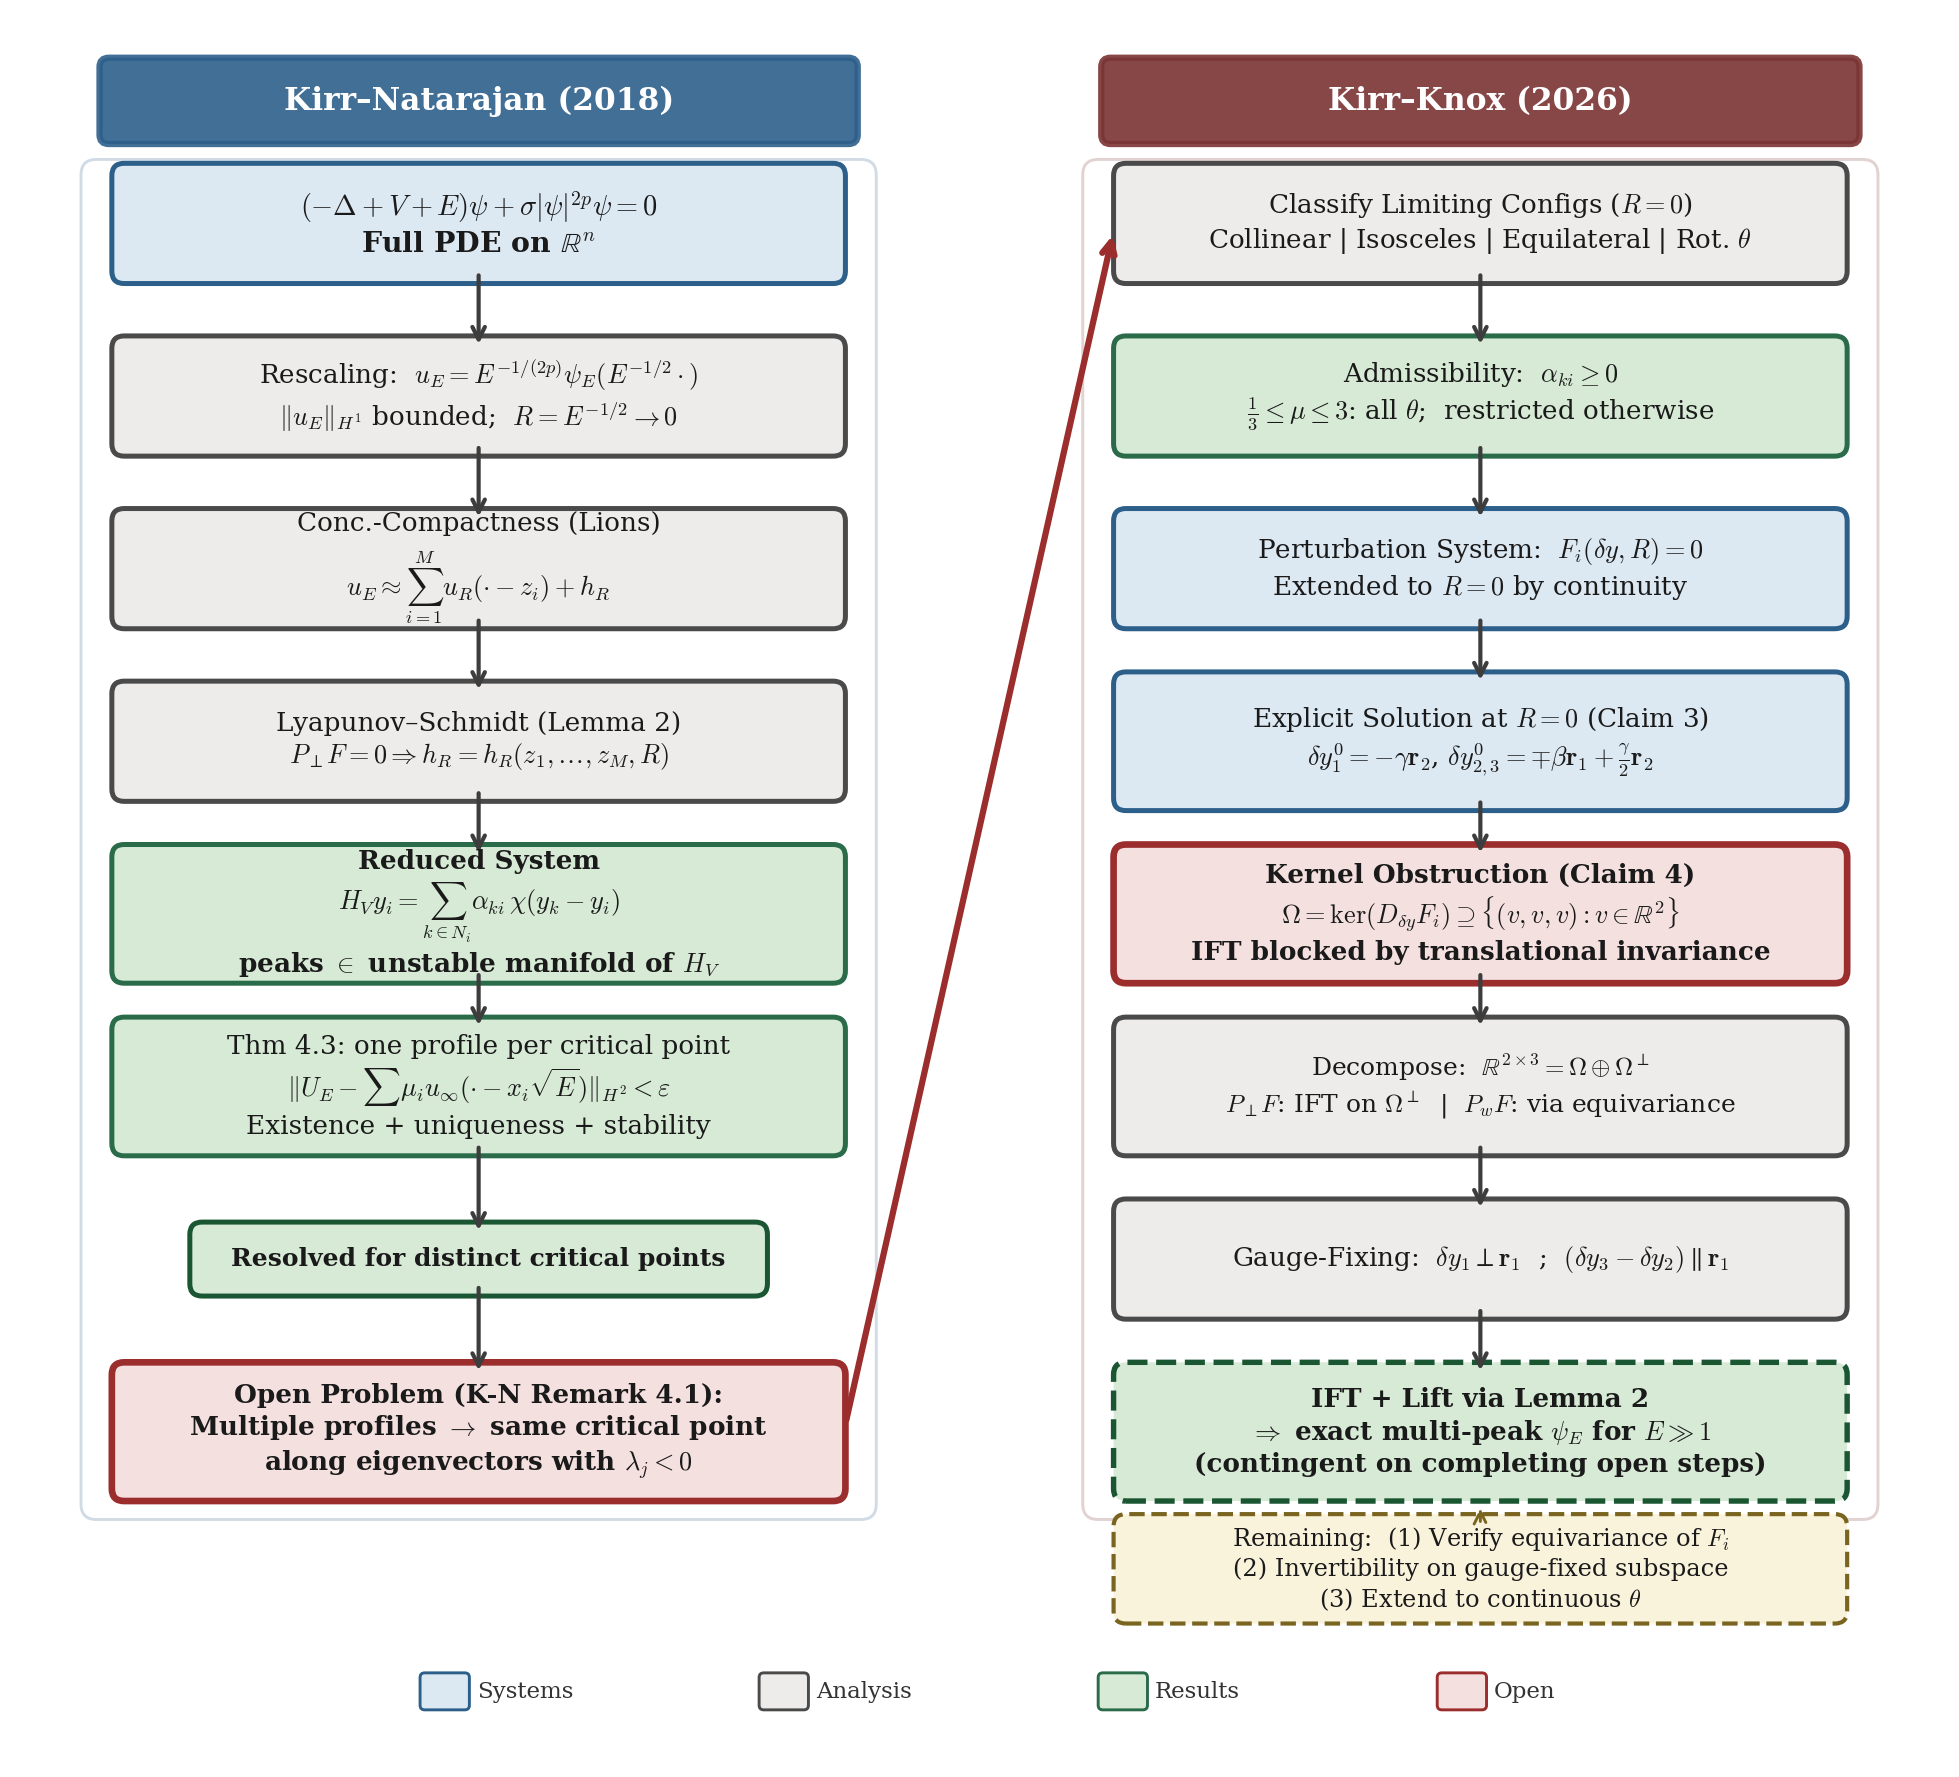
\includegraphics[width=1\linewidth]{../figures/figure_7_methodology_flowchart}
\caption{Complete analytical pipeline from the full PDE to the existence of
multi-peak ground states. The top portion (marked ``Kirr-Natarajan,
2018'') covers the rescaling, concentration-compactness decomposition,
and Lyapunov-Schmidt reduction established in \cite{KirrNatarajan2018}.
The lower portion (marked ``This work'') covers the classification
of admissible configurations, the perturbation system $F_{i}\left(\delta y,R\right)=0$,
the kernel obstruction and its resolution via gauge-fixing, and the
application of the implicit function theorem on the constrained subspace.
The open step (verifying rotational equivariance and invertibility
on the complement) is indicated at left.}
\label{fig:pipeline}
\end{figure}

Our contributions are threefold. First, we systematically classify
all admissible multi-peak configurations near a non-degenerate local
maximum of $V$ (Theorem~\ref{thm:classification}). Second, we formulate
and solve the perturbation system at $R=0$ (Proposition~\ref{prop:explicit-soln}),
identify the kernel obstruction (Proposition~\ref{prop:kernel}),
and propose a gauge-fixing strategy for its resolution (Section~\ref{sec:gauge}).
Third, we provide explicit admissibility regions in the $(\mu,\theta)$
parameter space for equilateral triangle configurations with rotational
freedom.

The multi-peak construction builds on a long line of work on semiclassical
and spike solutions of NLS. Floer and Weinstein~\cite{FloerWeinstein1986}
first proved the existence of standing waves concentrated near nondegenerate
critical points of $V$ for bounded potentials. The existence of ground
states for nonlinear scalar field equations was established by Berestycki
and Lions \cite{BerestyckiLions1983}, and the concentration compactness
framework for multi-peak decomposition was developed in~\cite{Lions1984a,Lions1984b},
and the symmetry-breaking bifurcation analysis for NLS with symmetric
potentials was carried out in~\cite{KirrKevrekidisPelinovsky2011}.
Stability of solitary waves under symmetry was established by Grillakis,
Shatah, and Strauss~\cite{GrillakisShatahStrauss1987,GrillakisShatahStrauss1990},
and asymptotic stability of ground states was proved in~\cite{KirrZarnescu2007,KirrMizrak2008}.
The present work extends the global bifurcation analysis of~\cite{KirrNatarajan2018}
by providing the first complete geometric classification of multi-peak
configurations and a systematic resolution strategy for the kernel
obstruction in the reduced system. Specifically, we carry out the
analysis identified as an open problem in Remark 4.1 of \cite{KirrNatarajan2018},
which notes that ``multiple profiles approaching the same critical
point along eigenvectors with negative eigenvalues'' requires a separate
treatment from the distinct-critical-point case resolved in their
Theorem 4.3.

\section{Setup and Preliminaries}

\label{sec:setup}

\subsection{Hypotheses on the potential}

\label{subsec:hypotheses}

We impose the following conditions on $V$, following~\cite{KirrKevrekidisPelinovsky2011,FloerWeinstein1986,KirrNatarajan2018}:

\begin{hyp}\label{hyp:V1} $V\in L^{\infty}(\R^{n})$, i.e., $V$
is bounded and measurable. \end{hyp}

\begin{hyp}\label{hyp:V2} ${\displaystyle \lim_{|x|\to\infty}V(x)=0}$.
\end{hyp}

\begin{hyp}\label{hyp:V3} $V$ is $C^{2}$ in a neighborhood of
$x_{0}$, where $x_{0}$ is a non-degenerate critical point of $V$:
$\nabla V(x_{0})=0$ and $\HV(x_{0})$ is invertible. \end{hyp}

\begin{hyp}\label{hyp:V4} All eigenvalues of $\HV(x_{0})$ are strictly
negative, i.e., $x_{0}$ is a strict local maximum of $V$. We write
$\lambda_{1},\ldots,\lambda_{n}<0$ for the eigenvalues with corresponding
orthonormal eigenvectors $\boldsymbol{r}_{1},\ldots,\boldsymbol{r}_{n}$.
\end{hyp}

Hypothesis~\ref{hyp:V1} ensures that $L_{0}=-\Delta+V$ is self-adjoint
on $L^{2}(\R^{n})$ with domain $H^{2}(\R^{n})$. Together with~\ref{hyp:V2},
it guarantees that the essential spectrum of $L_{0}$ is $[0,\infty)$
and that any negative eigenvalues are discrete. Hypothesis~\ref{hyp:V3}
is the minimal regularity needed for the Taylor expansion underlying
the Lyapunov--Schmidt reduction. Hypothesis~\ref{hyp:V4} is the
structural condition that forces multi-peak configurations to concentrate
at $x_{0}$; peaks at a local minimum would correspond to $\lambda_{i}>0$,
for which the algebraic system has no admissible solutions with $\alpha_{ki}\geq0$.

\begin{rmk} Floer and Weinstein~\cite{FloerWeinstein1986} work
with $V$ bounded and prove concentration near any nondegenerate critical
point (maximum or minimum). For the multi-peak case, the requirement
$\lambda_{i}<0$ arises from the interaction analysis: the peaks must
lie in the unstable subspace of $\HV(x_{0})$ (Corollary~\ref{cor:unstable}).
\end{rmk}

\subsection{Rescaling and concentration compactness}

\label{subsec:rescaling}

Following~\cite{KirrNatarajan2018}, define 
\begin{equation}
u_{E}(x)=E^{-\frac{1}{2p}}\,\psi_{E}(E^{-\frac{1}{2}}x),\label{eq:rescaling}
\end{equation}
so that $\norm{u_{E}}_{H^{1}}^{2}=\norm{\nabla\psi_{E}}_{L^{2}}^{2}+\norm{\psi_{E}}_{L^{2}}^{2}$
remains bounded. By the concentration compactness principle~\cite{Lions1984a},
there exists $M\in\N$ such that 
\begin{equation}
\norm{u_{E}(x)-\sum_{i=1}^{M}u_{i}(x-z_{i}(E))}_{H^{1}}\xrightarrow{E\to\infty}0,\label{eq:concentration}
\end{equation}
where each profile $u_{i}:\R^{n}\to\C$ solves the translation-invariant
equation 
\begin{equation}
(-\Delta+1)u+\sigma|u|^{2p}u=0.\label{eq:profile}
\end{equation}

\begin{figure}[H]
\centering
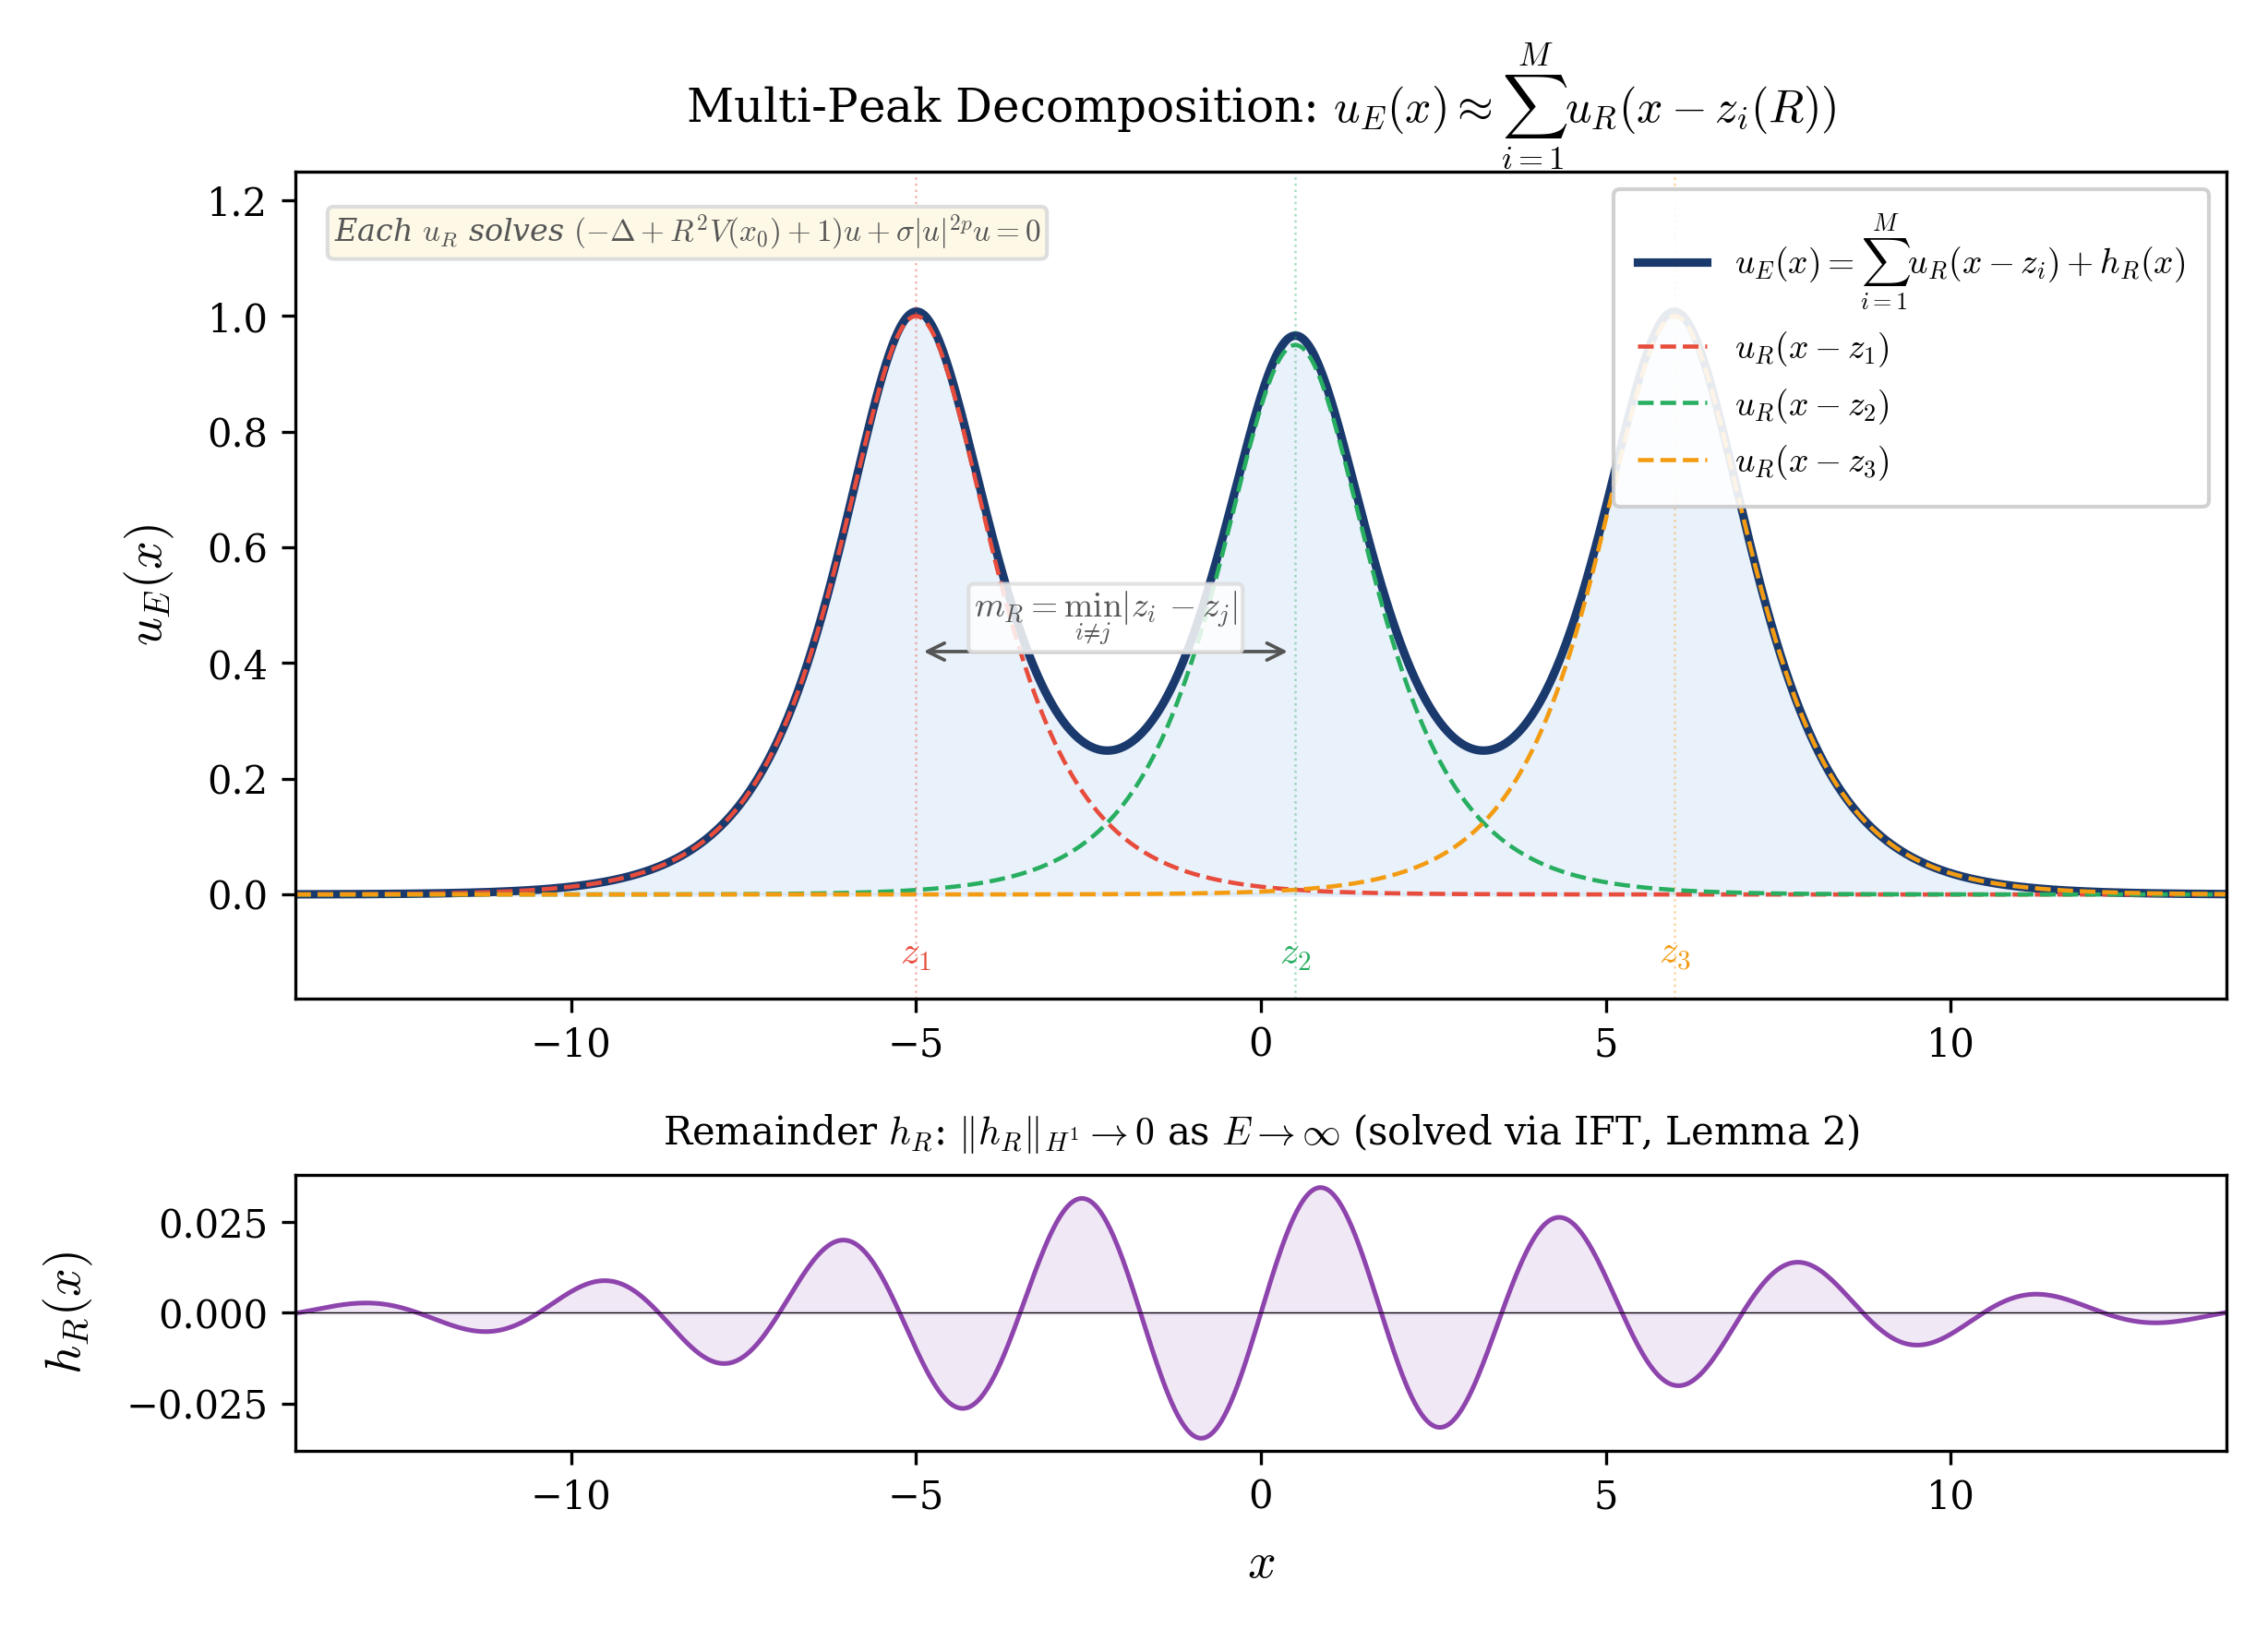
\includegraphics[width=0.75\linewidth]{../figures/figure_4_profile_decomposition}
\caption{Illustration of the concentration-compactness decomposition (\ref{eq:profile})
for $M=3$ peaks.\textbf{}\protect \\
\textbf{Top:} The rescaled solution $u_{E}\left(x\right)$ (solid
blue) is approximated by a sum of well-separated profiles $u_{R}\left(x-z_{i}\right)$
(dashed), each solving $\left(-\Delta+R^{2}V\left(x_{0}\right)+1\right)u+\sigma\left|u\right|^{2p}u=0$.
The minimum inter-peak distance $m_{R}=\min_{i\protect\neq j}\left|z_{i}-z_{j}\right|$
is indicated.\protect \\
\textbf{Bottom:} The remainder $h_{R}\left(x\right)$, which satisfies
$\left\Vert h_{R}\right\Vert _{H^{1}}\to0$ as $E\to\infty$ and is
recovered uniquely from the peak positions via the implicit function
theorem (\ref{lem:LS2}).}
\label{fig:decomposition}
\end{figure}

Setting $R=E^{-1/2}$, the rescaled NLS becomes 
\begin{equation}
(-\Delta+R^{2}V(Rx)+1)\,u_{E}+\sigma|u_{E}|^{2p}u_{E}=0.\label{eq:rescaled-NLS}
\end{equation}
Under Hypotheses~\ref{hyp:V1}--\ref{hyp:V2}, the rescaled peak
positions $Rz_{i}(R)$ remain bounded and converge to the critical
points of $V$ as $R\to0$.
\begin{prop}[{Kirr--Natarajan~\cite{KirrNatarajan2018}}]
\label{prop:convergence} Under Hypotheses~\ref{hyp:V1}--\ref{hyp:V4},
$Rz_{i}(R)\to x_{0}$ for each $i=1,\ldots,M$ as $R\to0$. 
\end{prop}
\begin{figure}[H]
\centering
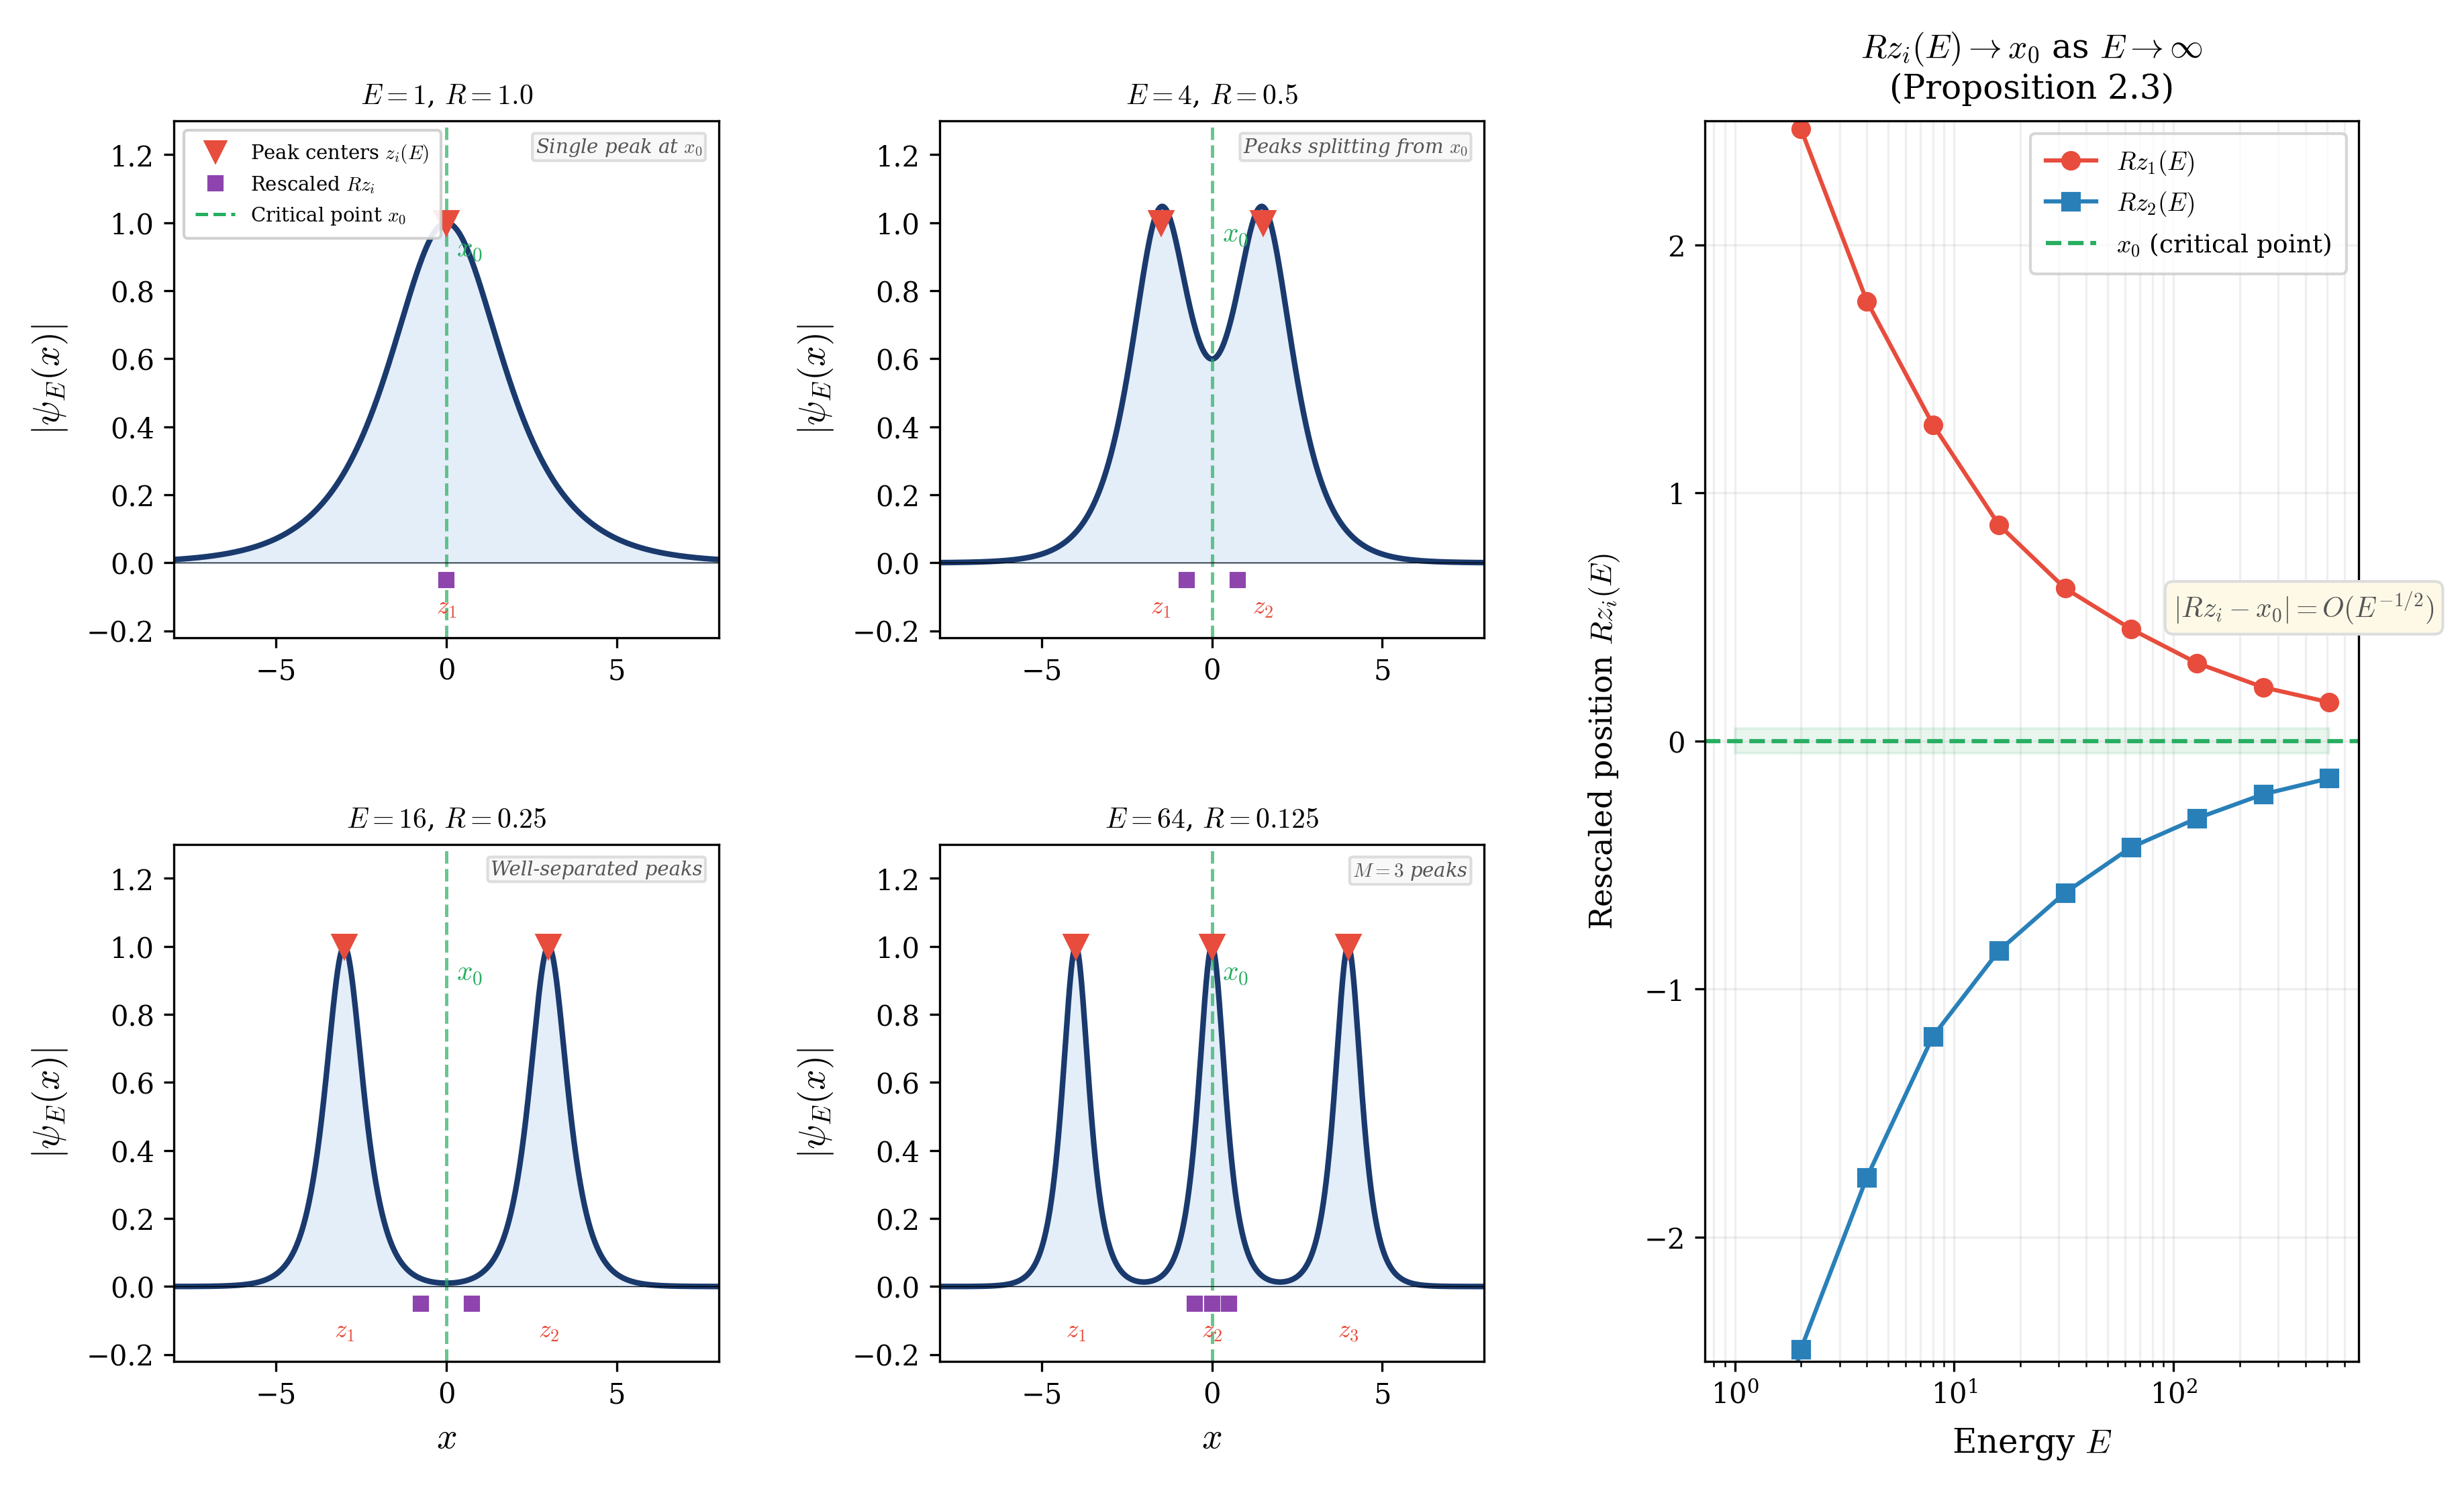
\includegraphics[width=0.75\linewidth]{../figures/figure_5_concentration_vs_peaks}
\caption{Evolution of peak structure with increasing energy $E$.\protect \\
\textbf{Left panels:} Profiles $\left|\psi_{E}\left(x\right)\right|$
at $E=1,4,16,64$, showing the transition from a single peak to well-separated
multi-peak structure. Red triangles mark the peak centers $z_{i}\left(E\right)$;
purple squares mark the rescaled positions $Rz_{i}$ converging toward
the critical point $x_{0}$ (green dashed line).\protect \\
\textbf{Right:} Convergence of $Rz_{i}\left(E\right)=E^{-\frac{1}{2}}z_{i}\left(E\right)$
to $x_{0}$ as $E\to\infty$, illustrating Proposition~\ref{prop:convergence}.
The convergence rate is $\left|Rz_{i}-x_{0}\right|=O\left(E^{-\frac{1}{2}}\right)$.}
\label{fig:concentration}
\end{figure}

We rewrite~(\ref{eq:concentration}) as 
\[
u_{E}(x)=\sum_{i=1}^{M}u_{R}(x-z_{i}(R))+h_{R}(x),
\]
where $u_{R}$ is the unique (up to phase) positive, spherically symmetric
solution of $(-\Delta+R^{2}V(x_{0})+1)u+\sigma|u|^{2p}u=0$.

\subsection{Lyapunov--Schmidt reduction}

\label{subsec:LS}

The derivatives $\partial u_{R}/\partial x_{j}$ satisfy the linearized
equation and generate the translational kernel. The Lyapunov-Schmidt
reduction proceeds in two steps:
\begin{lem}[{Lyapunov--Schmidt, Step 1~\cite{KirrNatarajan2018}}]
\label{lem:LS1} There exists $\varepsilon>0$ such that for $0<R<\varepsilon$,
there exist adjusted centers $\tilde{z}_{1},\ldots,\tilde{z}_{M}\in\R^{n}$
with $u_{E}(x)=\sum_{i=1}^{M}u_{R}(x-z_{i}(R))+\tilde{h}_{R}(x)$
and $\tilde{h}_{R}\perp\partial_{x_{j}}u_{R}(\cdot-z_{i}(R))$ for
all $i=1,\ldots,M$ and $j=1,\ldots,n$. 
\end{lem}
%
\begin{lem}[{Lyapunov--Schmidt, Step 2~\cite{KirrNatarajan2018}}]
\label{lem:LS2} There exist $\tilde{\varepsilon},\delta,d>0$ such
that if $R<\tilde{\varepsilon}$, $\norm{h}_{H^{1}}<\delta$, and
$|z_{i}-z_{j}|>d$ for $i\neq j$, then $P_{\perp}F(h,z_{1},\ldots,z_{M},R)=0$
has a unique solution $h=h(z_{1},\ldots,z_{M},R)$. 
\end{lem}

\subsection{The reduced algebraic system}

\label{subsec:reduced}

Projecting onto the translational modes yields the reduced system.
We introduce the following quantities:
\begin{defn}[Interaction functional and coefficients]
\label{def:interaction} The \emph{interaction functional} is 
\[
Q_{R}(z)=-\sigma\,\bigl\langle\partial_{z/|z|}u_{R}(\cdot-z),\,u_{R}^{2p+1}\bigr\rangle_{L^{2}}.
\]
The \emph{minimum inter-peak distance} is $m_{R}=\min\{|z_{j}(R)-z_{i}(R)|:i\neq j\}$.
The \emph{interaction coefficients} are 
\begin{equation}
\alpha_{ki}=\frac{Q_{R}(|z_{k}-z_{i}|)}{Q_{R}(m_{R})},\quad\text{satisfying }0\leq\alpha_{ki}\leq1,\label{eq:alpha-def}
\end{equation}
with $\alpha_{ki}=1$ precisely when $|z_{k}-z_{i}|=m_{R}$ (nearest
neighbors). 
\end{defn}
%
\begin{defn}[Overall interaction strength]
\label{def:chi} The \emph{overall interaction strength} is 
\begin{equation}
\chi=\frac{2\,Q_{R}(m_{R})}{\norm{u_{R}}_{L^{2}}^{2}\,R^{4}\,m_{R}}>0.\label{eq:chi-def}
\end{equation}
This is a single positive scalar that captures the magnitude of the
inter-peak interaction relative to the Hessian restoring force. It
is \emph{not} equal to any individual $\alpha_{ki}$; rather, the
force on peak $i$ from peak $k$ has magnitude $\alpha_{ki}\chi$. 
\end{defn}
\begin{figure}[H]
\centering
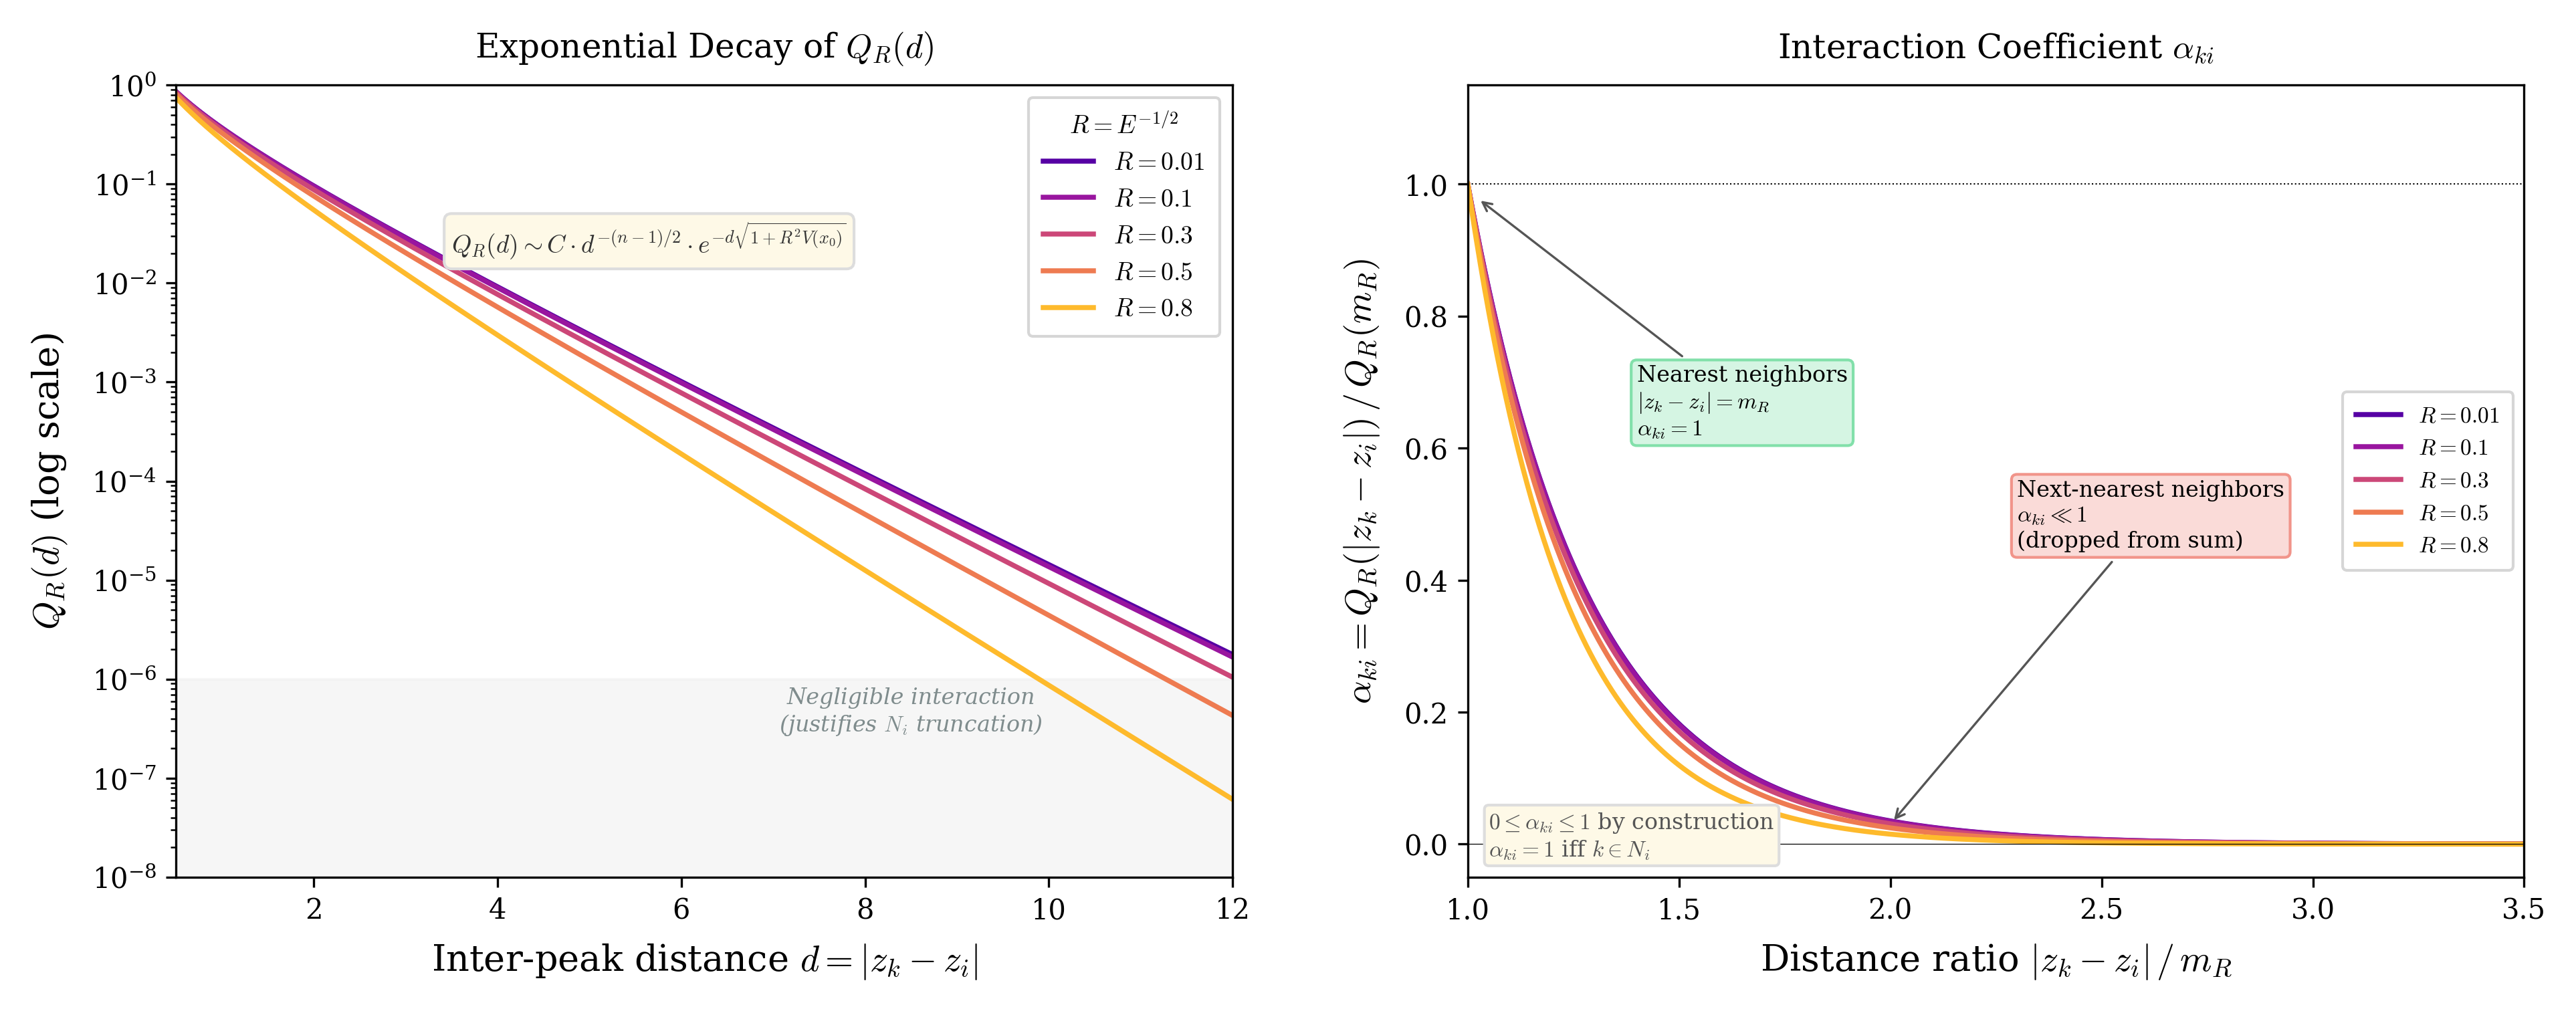
\includegraphics[width=0.75\linewidth]{../figures/figure_6_interaction_decay}
\caption{\textbf{(a)} Semilog plot of the interaction functional $Q_{R}\left(d\right)=-\sigma\left\langle \partial_{\hat{d}}u_{R}\left(\cdot-d\right),u_{R}^{2p+1}\right\rangle $
as a function of inter-peak distance $d$ for several values of $R=E^{-\frac{1}{2}}$.
The exponential decay $Q_{R}\left(d\right)\sim C\cdot d^{-\frac{n-1}{2}}\cdot e^{-d\sqrt{1+R^{2}V\left(x_{0}\right)}}$
ensures that only nearest-neighbor interactions contribute at leading
order, justifying the truncation of the sum to $k\in N_{i}$.\textbf{}\protect \\
\textbf{(b)} The interaction coefficient $\alpha_{ki}=\frac{Q_{R}\left(\left|z_{k}-z_{i}\right|\right)}{Q_{R}\left(m_{R}\right)}$
as a function of the distance ratio $\frac{\left|z_{k}-z_{i}\right|}{m_{R}}$.
By construction $0\protect\leq\alpha_{ki}\protect\leq1$, with $\alpha_{ki}=1$
for nearest neighbors ($\left|z_{k}-z_{i}\right|=m_{R}$) and $\alpha_{ki}\ll1$
for next-nearest neighbors, which are dropped from the reduced system.}
\label{fig:interaction}
\end{figure}

The orthogonality condition from the Lyapunov--Schmidt projection
yields, after the rescaling $s_{i}=Rz_{i}-x_{0}$ and passage to the
limit $R\to0$ with $y_{i}=\lim_{R\to0}\frac{s_{i}}{Rm_{R}}$: 
\begin{equation}
\HV(x_{0})\,y_{i}=\chi\sum_{k\in N_{i}}\alpha_{ki}(y_{k}-y_{i}),\label{eq:algebraic}
\end{equation}
where $N_{i}=\{k:|y_{k}-y_{i}|=1\}$ is the set of nearest neighbors
and we have used $|y_{k}-y_{i}|=1$ for nearest neighbors.
\begin{cor}
\label{cor:unstable} The peak positions satisfy $\operatorname{span}\{y_{1},\ldots,y_{M}\}\subseteq U$,
where 
\[
U=\operatorname{span}\bigl\{\boldsymbol{r}\in\R^{n}:\HV(x_{0})\boldsymbol{r}=\lambda\boldsymbol{r},\;\lambda<0\bigr\}
\]
is the unstable subspace of $\HV(x_{0})$. 
\end{cor}
\begin{proof}
Write $y_{i}=y_{i}^{U}+y_{i}^{S}$ with $y_{i}^{U}\in U$ and $y_{i}^{S}\in U^{\perp}$.
Applying the orthogonal projection $P_{S}$ onto $U^{\perp}$ to the
algebraic system~(\ref{eq:algebraic}) gives 
\begin{equation}
\HV\,y_{i}^{S}=\chi\sum_{k\in N_{i}}\alpha_{ki}\bigl(y_{k}^{S}-y_{i}^{S}\bigr),\label{eq:projected-stable}
\end{equation}
since $\HV$ preserves both $U$ and $U^{\perp}$ (they are eigenspaces)
and $P_{S}(y_{k}-y_{i})=y_{k}^{S}-y_{i}^{S}$.

Now take the inner product of~(\ref{eq:projected-stable}) with $y_{i}^{S}$
and sum over~$i$: 
\[
\sum_{i=1}^{M}\ip{y_{i}^{S}}{\HV\,y_{i}^{S}}=\chi\sum_{i=1}^{M}\sum_{k\in N_{i}}\alpha_{ki}\,\ip{y_{i}^{S}}{y_{k}^{S}-y_{i}^{S}}.
\]
\textbf{Left side.} Since $\HV\big|_{U^{\perp}}$ has all eigenvalues
in $[\lambda_{\min}^{S},\infty)$ with $\lambda_{\min}^{S}>0$ (Hypothesis~V4
places the peaks at a strict local maximum, so eigenvalues in directions
\emph{not} used by the peaks are positive), we have 
\[
\text{LHS}\;\geq\;\lambda_{\min}^{S}\sum_{i}\abs{y_{i}^{S}}^{2}.
\]
\textbf{Right side.} Each nearest-neighbor edge $\{i,k\}$ contributes
the ordered pairs $(i,k)$ and $(k,i)$. Using the symmetry $\alpha_{ki}=\alpha_{ik}$
(since $Q_{R}$ depends only on $\abs{z_{k}-z_{i}}$), the contribution
of each edge is 
\begin{align*}
\alpha_{ki}\Bigl[\ip{y_{i}^{S}}{y_{k}^{S}-y_{i}^{S}}+\ip{y_{k}^{S}}{y_{i}^{S}-y_{k}^{S}}\Bigr] & =-\alpha_{ki}\abs{y_{k}^{S}-y_{i}^{S}}^{2}.
\end{align*}
Summing over all edges: 
\[
\text{RHS}=-\chi\!\!\sum_{\{i,k\}\in\text{edges}}\alpha_{ki}\abs{y_{k}^{S}-y_{i}^{S}}^{2}\;\leq\;0,
\]
since $\chi>0$ and every $\alpha_{ki}\geq0$.

Combining: $\lambda_{\min}^{S}\sum_{i}\abs{y_{i}^{S}}^{2}\leq0$.
Because $\lambda_{\min}^{S}>0$, we conclude $y_{i}^{S}=0$ for every
$i=1,\ldots,M$. 
\end{proof}

\section{Classification of Limiting Configurations}

\label{sec:classification}

We now classify all admissible solutions of the algebraic system~(\ref{eq:algebraic})
for peaks lying in the plane spanned by two eigenvectors $\boldsymbol{r}_{1},\boldsymbol{r}_{2}$
of $\HV(x_{0})$, with eigenvalues $\lambda_{1},\lambda_{2}<0$.

\begin{figure}[H]
\centering
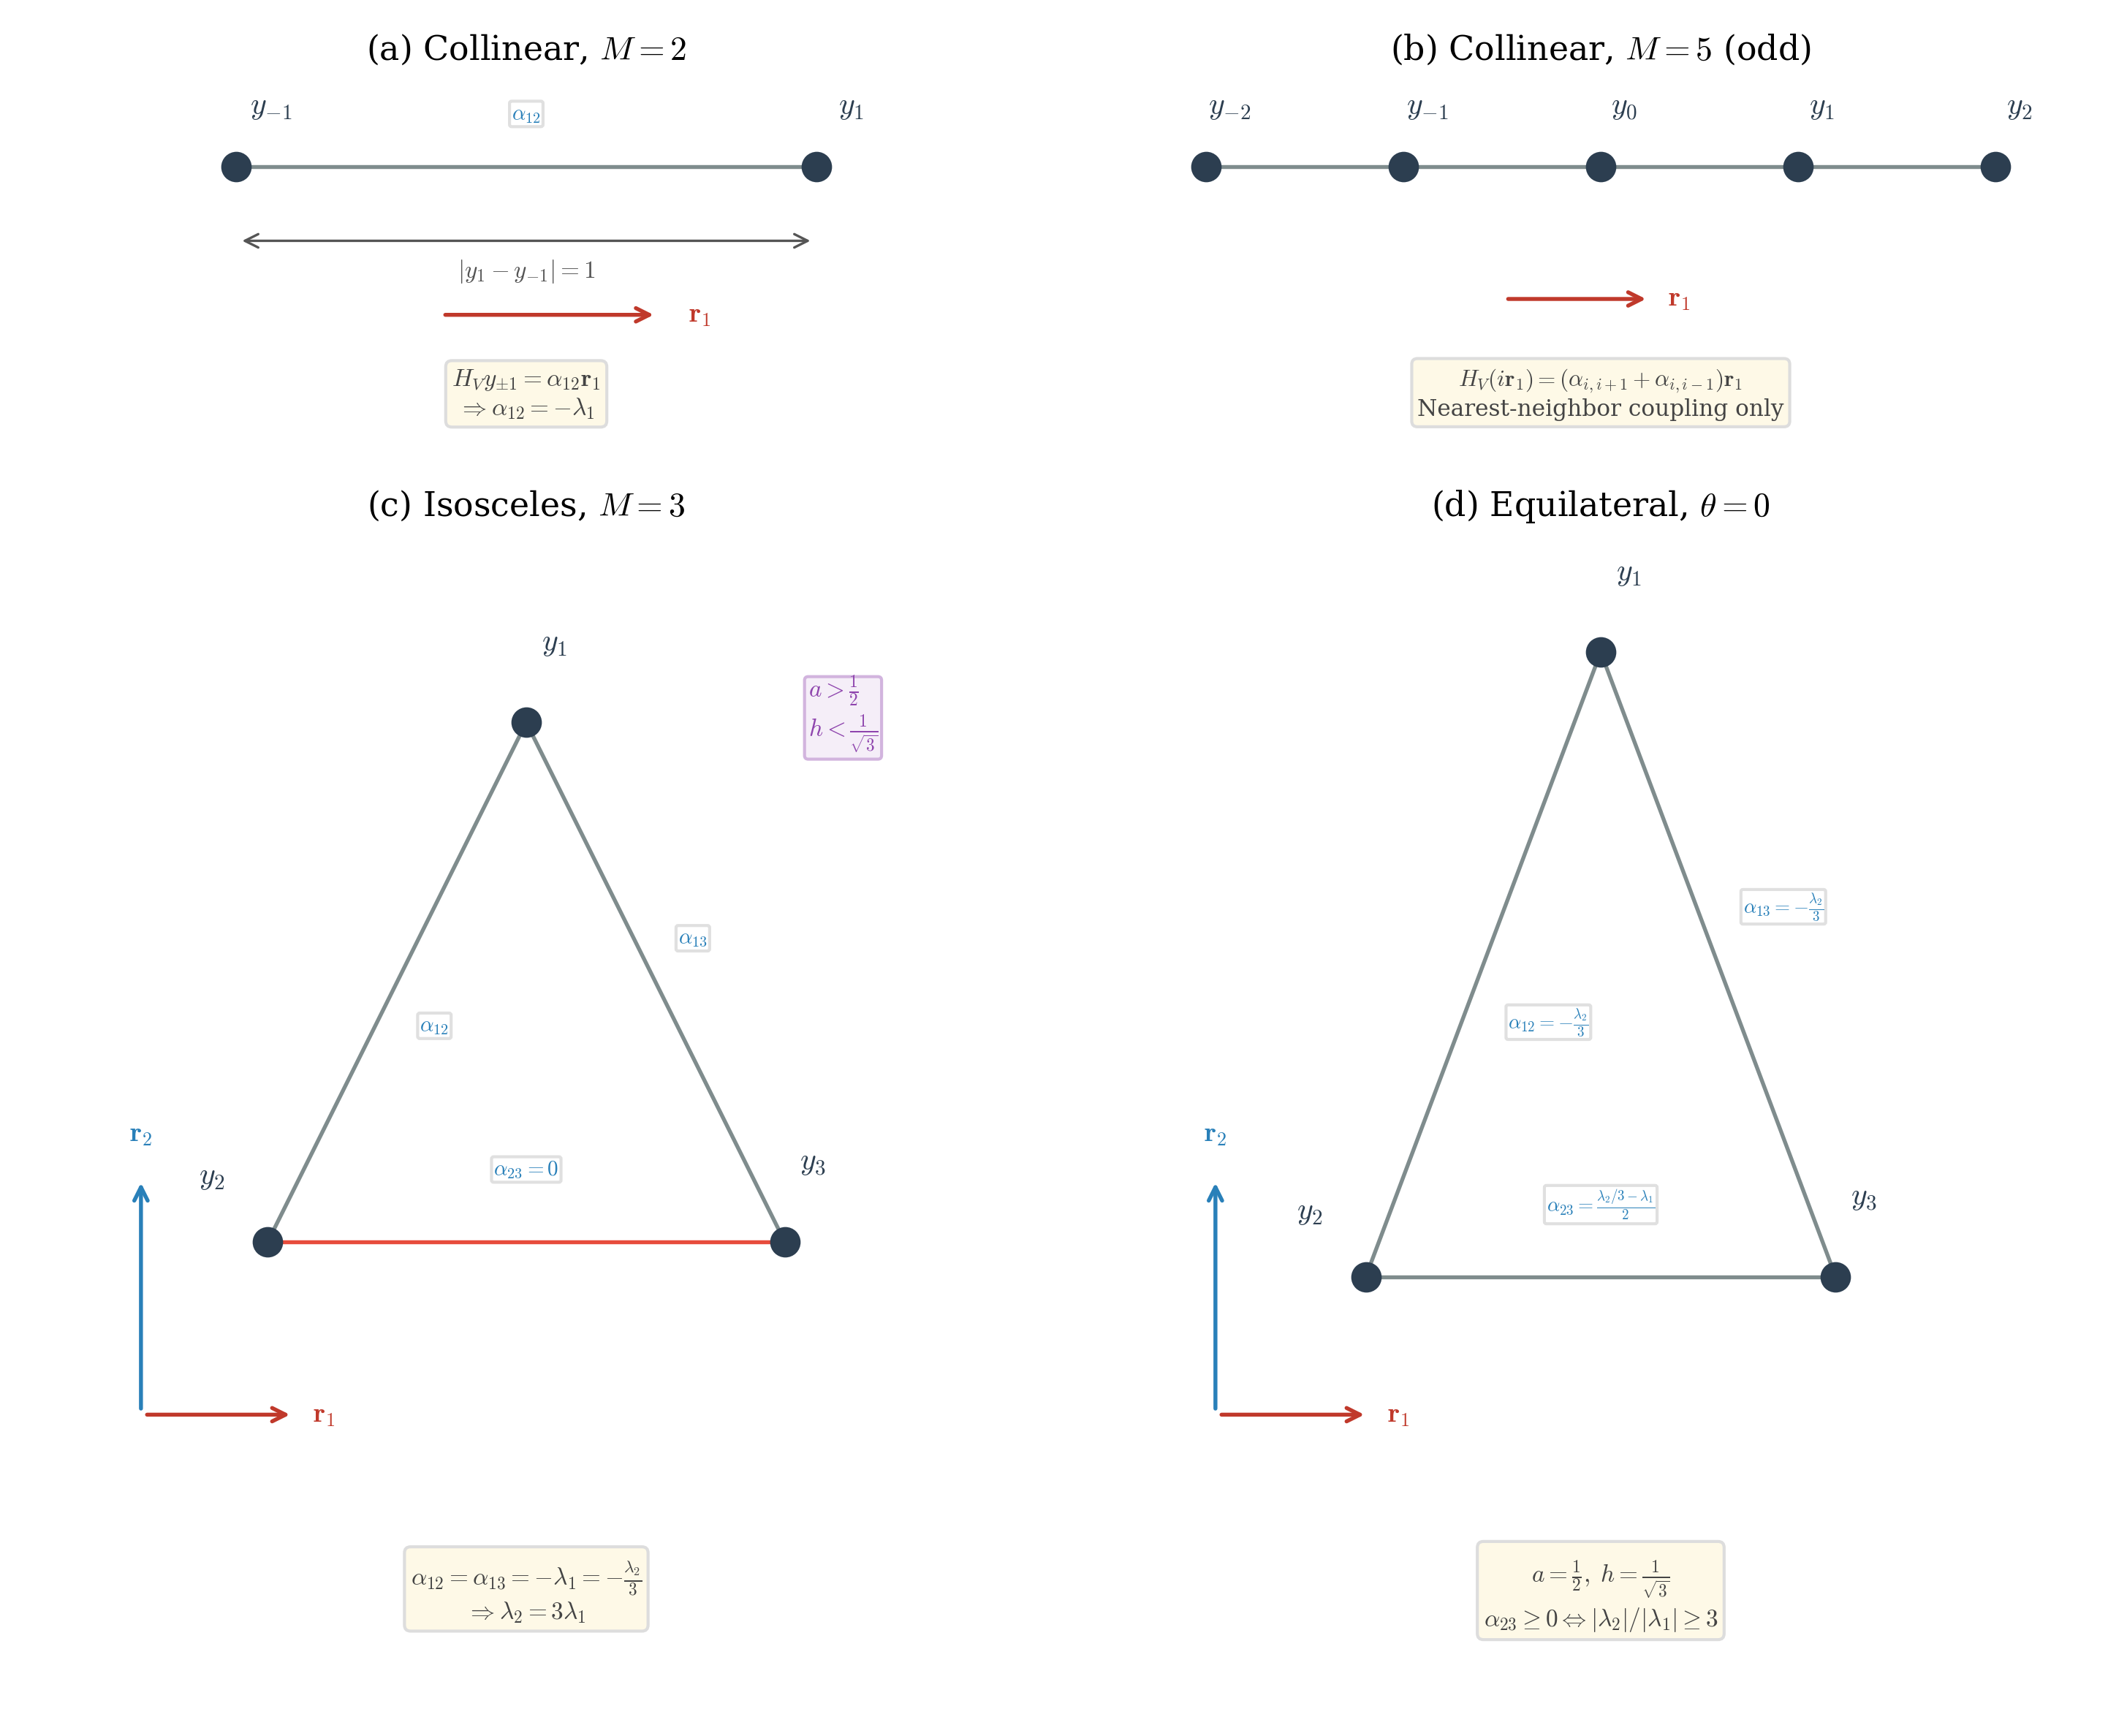
\includegraphics[width=0.75\linewidth]{../figures/figure_2_peak_configurations}
\caption{Schematic representations of the admissible multi-peak configurations
classified in Section~\ref{sec:classification}.\protect \\
\textbf{(a)} Collinear arrangement with $M=2$ peaks along the eigenvector
$\boldsymbol{r}_{1}$ of $H_{V}$; the reduced system yields $\alpha_{12}=-\lambda_{1}$.
\textbf{}\protect \\
\textbf{(b)} Collinear arrangement with \$M=5\$ (odd) peaks; the nearest-neighbor
coupling structure $H_{V}(i\boldsymbol{r}_{1})=(\alpha_{i,i+1}+\alpha_{i,i-1})\boldsymbol{r}_{1}$
is indicated.\textbf{}\protect \\
\textbf{(c)} Isosceles triangle ($a>\frac{1}{2}$, $h<\frac{1}{\sqrt{3}}$)
in the plane spanned by $\boldsymbol{r}_{1},\boldsymbol{r}_{2}$,
with $\alpha_{23}=0$ (base edge decoupled) and the constraint $\lambda_{2}=3\lambda_{1}$.\textbf{}\protect \\
\textbf{(d)} Equilateral triangle at $\theta=0$ with explicit $\alpha$
values; the admissibility condition $\alpha_{23}\protect\geq0$ is
equivalent to $\frac{\left|\lambda_{2}\right|}{\left|\lambda_{1}\right|}\protect\geq3$.}
\label{fig:configurations}
\end{figure}
\begin{figure}[H]
\centering
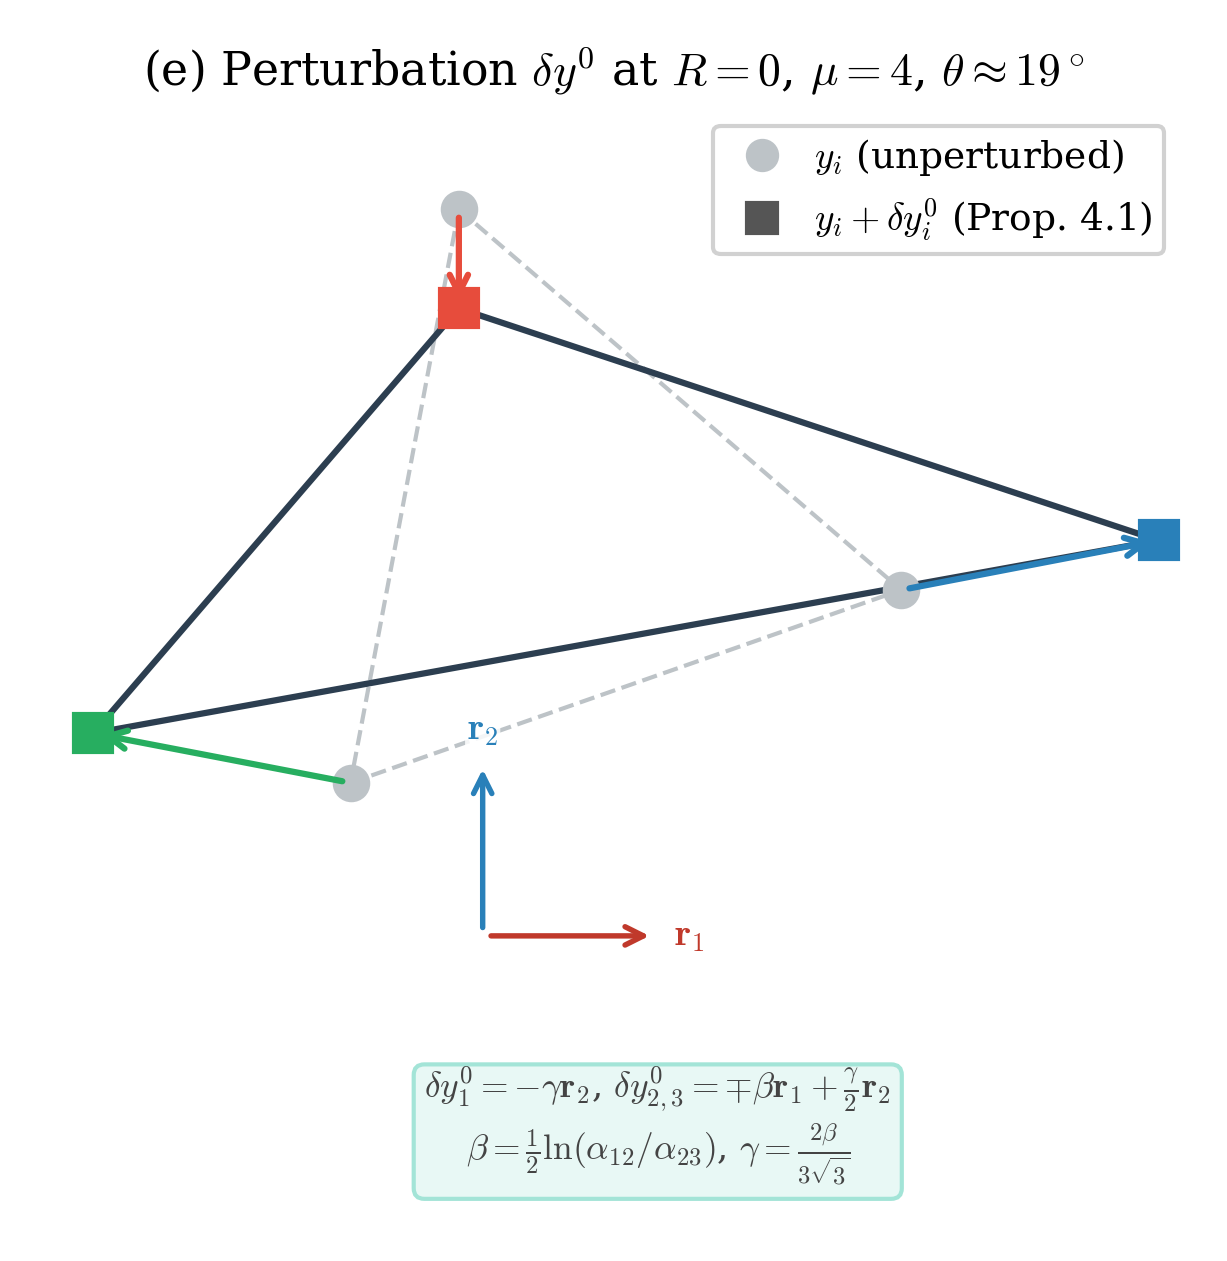
\includegraphics[width=0.5\linewidth]{../figures/figure_2b_perturbation}

\caption{The perturbation $\delta y^{0}$ (Proposition \ref{prop:explicit-soln})
at $R=0$ for the rotated equilateral triangle at $\mu=4$, $\theta\approx19^{\circ}$
(an admissible point in the $\left(\mu,\theta\right)$ phase diagram
of Figure \ref{fig:admissibility}). Gray circles mark the unperturbed
peak positions $y_{i}$; colored squares mark the perturbed positions
$y_{i}+\delta y_{i}^{0}$, with arrows indicating the displacement
vector. The parameters $\beta=\frac{1}{2}\ln\left(\frac{\alpha_{12}}{\alpha_{23}}\right)$
and $\gamma=\frac{2\beta}{3\sqrt{3}}$ are derived from the requirement
that $\tilde{\alpha}_{12}=\tilde{\alpha}_{13}=1$. Note that the equilateral
configuration at $\theta=0$ has $\alpha_{23}\protect\leq0$ for $\mu>3$,
so a nonzero rotation angle is needed for the perturbation formula
to apply.}

\label{fig:perturbation}
\end{figure}

\begin{thm}[Classification of admissible multi-peak configurations]
\label{thm:classification} Under Hypotheses~\ref{hyp:V1}--\ref{hyp:V4},
the admissible solutions of~(\ref{eq:algebraic}) with all $\alpha_{ki}\geq0$
are: 
\begin{enumerate}
\item[(a)] \textbf{Collinear} ($M\geq2$): All peaks aligned along a single
eigenvector $\boldsymbol{r}_{1}$ of $\HV(x_{0})$. 
\item[(b)] \textbf{Isosceles triangle} ($M=3$): Peaks in the $(\boldsymbol{r}_{1},\boldsymbol{r}_{2})$-plane
with $\alpha_{12}=\alpha_{13}=-\lambda_{2}/3$ and the eigenvalue
constraint $\lambda_{2}=3\lambda_{1}$. 
\item[(c)] \textbf{Equilateral triangle} ($M=3$): Peaks at unit mutual distance
with $\alpha_{12}=\alpha_{13}=-\frac{\lambda_{2}}{3}$, $\alpha_{23}=\frac{\lambda_{2}}{6}-\frac{\lambda_{1}}{2}$,
requiring $\frac{\left|\lambda_{2}\right|}{\left|\lambda_{1}\right|}\geq3$. 
\item[(d)] \textbf{Rotational equilateral} ($M=3$, angle $\theta$): The equilateral
triangle rotated by angle $\theta$ relative to the eigenvector basis.
The admissible $(\mu,\theta)$ regions, where $\mu=\frac{\left|\lambda_{2}\right|}{\left|\lambda_{1}\right|}$,
are given by Table~\ref{tab:summary}. 
\end{enumerate}
\end{thm}
The proof of Theorem~\ref{thm:classification} occupies the remainder
of this section.

\noindent\begin{rmk}[Convention for interaction coefficients in
the classification]\label{rmk:alpha-convention} In the proofs of
Theorem~\ref{thm:classification} that follow, the algebraic system~(\ref{eq:algebraic})
is written in the absorbed form 
\begin{equation}
\HV(x_{0})\,y_{i}=\sum_{k\in N_{i}}\hat{\alpha}_{ki}(y_{k}-y_{i}),\quad\hat{\alpha}_{ki}\geq0,\label{eq:algebraic-absorbed}
\end{equation}
where $\hat{\alpha}_{ki}=\alpha_{ki}\chi$ is the \emph{combined force
coefficient}, incorporating the overall interaction strength $\chi$
from Definition~\ref{def:chi}. This convention avoids carrying $\chi$
through the algebraic manipulations.

\smallskip{}
To recover the normalized coefficients of Definition~\ref{def:interaction}
(satisfying $0\leq\alpha_{ki}\leq1$ with $\alpha_{ki}=1$ at minimum
distance), one divides by $\chi$: 
\[
\alpha_{ki}=\frac{\hat{\alpha}_{ki}}{\chi},\qquad\chi=\max_{k,i}\hat{\alpha}_{ki}.
\]

\smallskip{}
\textbf{Example: equilateral triangle at $\theta=0$.} The proofs
below yield $\hat{\alpha}_{12}=\hat{\alpha}_{13}=-\frac{\lambda_{2}}{3}$
and $\hat{\alpha}_{23}=\frac{\lambda_{2}}{6}-\frac{\lambda_{1}}{2}$.
Since $\hat{\alpha}_{12}=\hat{\alpha}_{13}\geq\hat{\alpha}_{23}$
for $\mu\geq3$ (with equality only at $\mu=3$), the overall interaction
strength is 
\[
\chi=\hat{\alpha}_{12}=-\frac{\lambda_{2}}{3}>0,
\]
and the normalized base-edge coefficient is 
\[
\alpha_{23}=\frac{\hat{\alpha}_{23}}{\chi}=\frac{\frac{\lambda_{2}}{6}-\frac{\lambda_{1}}{2}}{-\frac{\lambda_{2}}{3}}=1-\frac{3}{2\mu}\;\in\;[0,1).
\]
In particular, $\alpha_{23}<1$ for $\mu>3$, reflecting the fact
that the base edge is \emph{not} at the minimum inter-peak distance:
the perturbation $\delta y^{0}$ of Proposition~\ref{prop:explicit-soln}
pushes the base vertices slightly apart relative to the apex--base
edges. \end{rmk}

\subsection{Collinear configurations}

\label{subsec:collinear}
\begin{proof}[Proof of Theorem~\ref{thm:classification}(a)]
Let $y_{i}$ be $M$ connected collinear points along $\boldsymbol{r}_{1}$.
For $M$ even, set $y_{\pm i}=\pm(i-\frac{1}{2})\boldsymbol{r}_{1}$;
for $M$ odd, set $y_{0}=0$, $y_{\pm i}=\pm i\,\boldsymbol{r}_{1}$.
The nearest-neighbor constraint gives 
\[
\HV\,y_{i}=(\alpha_{i,i+1}+\alpha_{i,i-1})\boldsymbol{r}_{1}
\]
with $\alpha_{i,i\pm1}\geq0$ determined recursively. Since $\boldsymbol{r}_{1}$
is an eigenvector with $\lambda_{1}<0$, each equation reduces to
a scalar relation $\lambda_{1}c_{i}=\chi(\alpha_{i,i+1}+\alpha_{i,i-1})$
with $c_{i}$ the coefficient of $y_{i}$ along $\boldsymbol{r}_{1}$.
The non-negativity $\alpha\geq0$ is guaranteed by $\lambda_{1}<0$
and $\chi>0$. 
\end{proof}

\subsection{Isosceles triangle}

\label{subsec:isosceles}
\begin{proof}[Proof of Theorem~\ref{thm:classification}(b)]
Let $y_{1}=\left(0,h\right)^{\intercal}$, $y_{2}=\left(-a,-\frac{h}{2}\right)^{\intercal}$,
$y_{3}=\left(a,-\frac{h}{2}\right)^{\intercal}$ with $2a>1$ (so
$|y_{2}-y_{3}|=2a>1$ and the nearest-neighbor pairs are $(1,2)$
and $(1,3)$ only) and the geometric constraint $a^{2}+\left(\frac{3h}{2}\right)^{2}=1$.

From the equation for $y_{1}$: 
\begin{align*}
\HV y_{1} & =\alpha_{12}(y_{2}-y_{1})+\alpha_{13}(y_{3}-y_{1})\\
(0,\lambda_{2}h)^{\intercal} & =\bigl(a(\alpha_{13}-\alpha_{12}),\;-\frac{3h}{2}(\alpha_{13}+\alpha_{12})\bigr)^{\intercal},
\end{align*}
which gives $\alpha_{12}=\alpha_{13}=-\lambda_{2}/3$.

From the equation for $y_{2}$ (with only $y_{1}$ as nearest neighbor):
$\HV y_{2}=\alpha_{12}(y_{1}-y_{2})$, yielding component-wise $-a\lambda_{1}=a\alpha_{12}$
and $-(h/2)\lambda_{2}=(3h/2)\alpha_{12}$. The first gives $\alpha_{12}=-\lambda_{1}$
and the second $\alpha_{12}=-\lambda_{2}/3$, hence $\lambda_{2}=3\lambda_{1}$. 
\end{proof}

\subsection{Equilateral triangle}

\label{subsec:equilateral}
\begin{proof}[Proof of Theorem~\ref{thm:classification}(c)]
Set $2a=1$, giving $a=\frac{1}{2}$, $h=\frac{1}{\sqrt{3}}$, and
$|y_{k}-y_{i}|=1$ for all pairs. All three pairs are nearest neighbors.
From $y_{1}$: $\alpha_{12}=\alpha_{13}=-\frac{\lambda_{2}}{3}$ as
before. From $y_{2}$ (with both $y_{1}$ and $y_{3}$ as neighbors):
\begin{align*}
\HV y_{2} & =\alpha_{12}(y_{1}-y_{2})+\alpha_{23}(y_{3}-y_{2}),\\
(-a\lambda_{1},\,-\frac{h}{2}\lambda_{2})^{\intercal} & =(a\alpha_{12}+2a\alpha_{23},\;\frac{3h}{2}\alpha_{12})^{\intercal},
\end{align*}
giving $\alpha_{23}=\frac{\lambda_{2}}{6}-\frac{\lambda_{1}}{2}$.
The constraint $\alpha_{23}\geq0$ requires $\lambda_{2}\geq3\lambda_{1}$,
i.e., $\frac{\left|\lambda_{2}\right|}{\left|\lambda_{1}\right|}\geq3$. 
\end{proof}

\subsection{Rotational equilateral triangle}

\label{subsec:rotational}
\begin{proof}[Proof of Theorem~\ref{thm:classification}(d)]
Let $R(\theta)$ be the $2\times2$ rotation matrix by angle $\theta$
and set $y_{i}=R(\theta)y_{i}'$ where $y_{i}'$ are the canonical
equilateral positions. The conjugated Hessian $\tilde{H}=R(-\theta)\HV R(\theta)$
has entries 
\[
\tilde{H}=\begin{pmatrix}\lambda_{1}\cos^{2}\theta+\lambda_{2}\sin^{2}\theta & (\lambda_{2}-\lambda_{1})\sin\theta\cos\theta\\
(\lambda_{2}-\lambda_{1})\sin\theta\cos\theta & \lambda_{2}\cos^{2}\theta+\lambda_{1}\sin^{2}\theta
\end{pmatrix}.
\]
Solving $\tilde{H}\,y_{i}'=\sum_{k\in N_{i}}\alpha_{ki}(y_{k}'-y_{i}')$
for each vertex yields the $\theta$-dependent coefficients: 
\begin{align}
\alpha_{12}(\theta) & =\frac{1}{3}\bigl[\lambda_{2}(-\sqrt{3}\sin\theta-\cos\theta)\cos\theta+\lambda_{1}(-\sin\theta+\sqrt{3}\cos\theta)\sin\theta\bigr],\label{eq:alpha12}\\
\alpha_{13}(\theta) & =\frac{1}{3}\bigl[\lambda_{2}(\sqrt{3}\sin\theta-\cos\theta)\cos\theta-\lambda_{1}(\sin\theta+\sqrt{3}\cos\theta)\sin\theta\bigr],\label{eq:alpha13}\\
\alpha_{23}(\theta) & =\frac{1}{6}\bigl[\lambda_{2}(2\cos2\theta-1)-\lambda_{1}(2\cos2\theta+1)\bigr].\label{eq:alpha23}
\end{align}
\end{proof}
\begin{figure}[H]
\centering
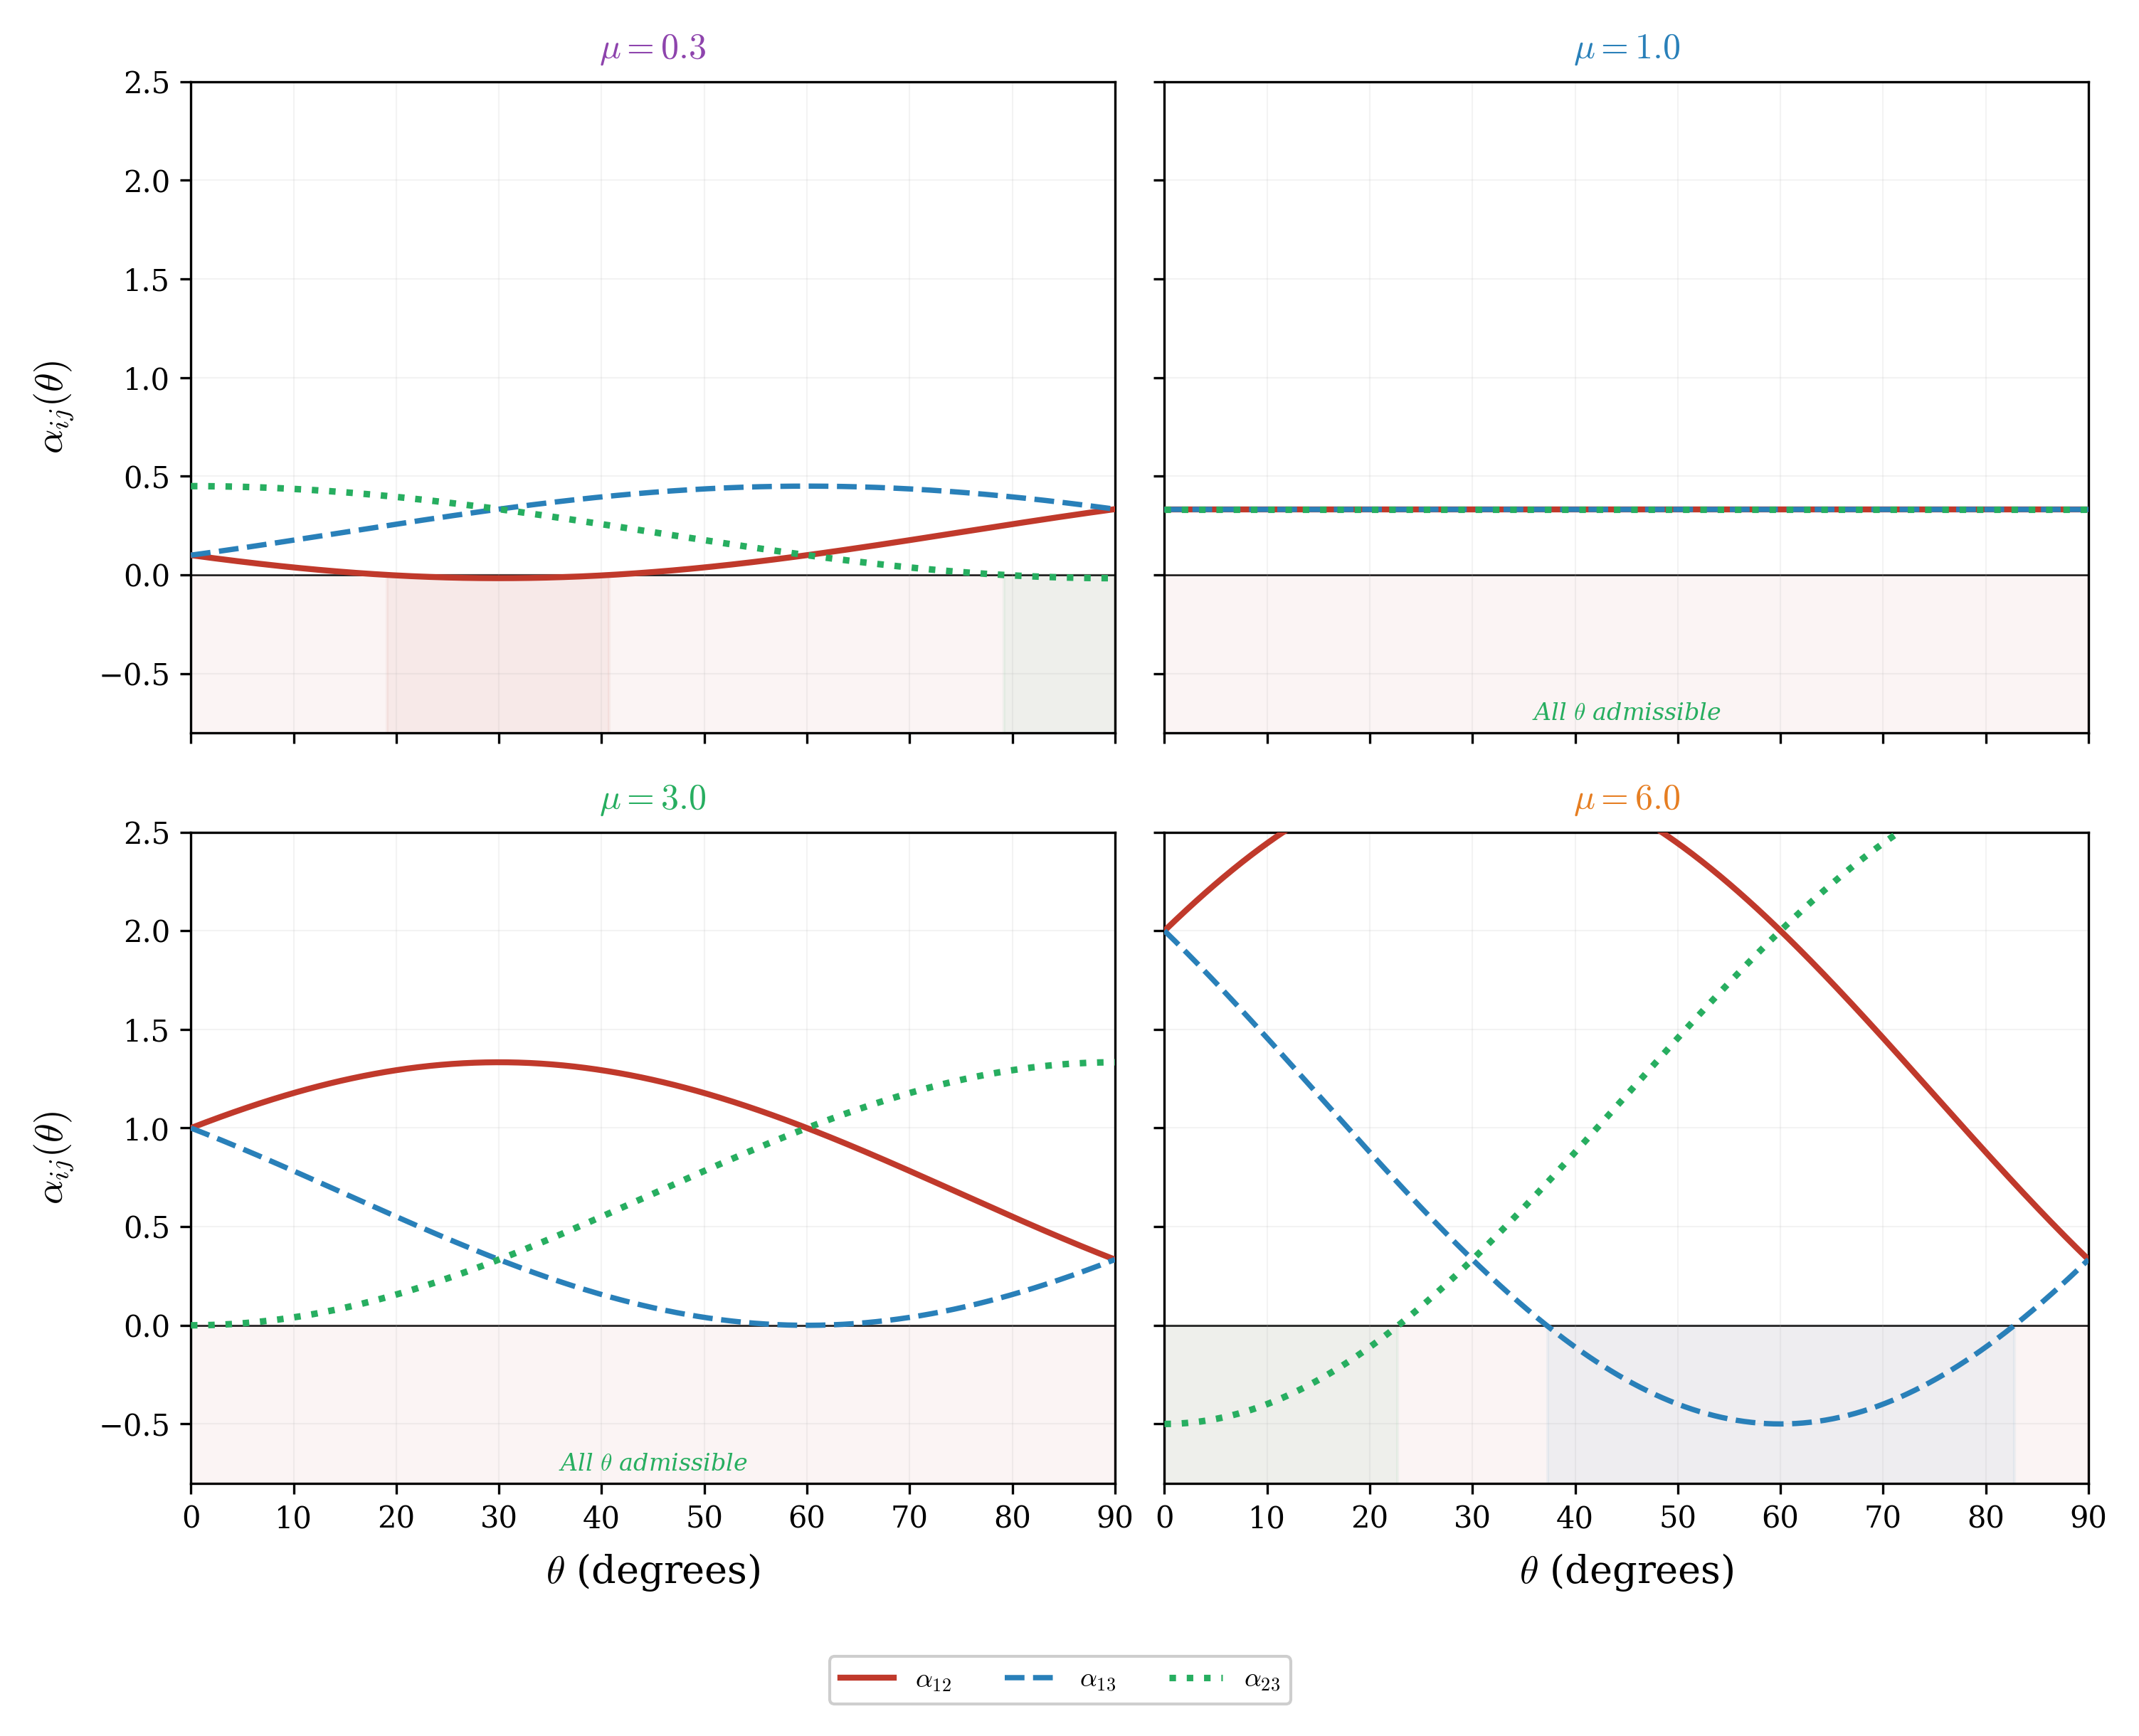
\includegraphics[width=0.75\linewidth]{../figures/figure_3_alpha_vs_theta_vs_mu}
\caption{Dependence of the interaction coefficients $\alpha_{12}\left(\theta\right)$,
$\alpha_{13}\left(\theta\right)$, and $\alpha_{23}\left(\theta\right)$
on the rotation angle $\theta$ for six values of the eigenvalue ratio
$\mu\in\left\{ \frac{1}{5},\frac{1}{2},1,2,3,5\right\} $. Each coefficient
is computed from the expressions derived in Section~\ref{subsec:rotational}
(equations for $\alpha_{12}$, $\alpha_{13}$, $\alpha_{23}$ as functions
of $\lambda_{1}$, $\lambda_{2}$, and $\theta$). The shaded region
$\alpha<0$ is forbidden by the physical requirement that inter-peak
interactions be attractive for the focusing nonlinearity ($\sigma>0$).
Physical interpretation: $\alpha_{12}$ quantifies the apex-to-base-left
coupling, $\alpha_{13}$ the apex-to-base-right coupling, and $\alpha_{23}$
the base edge coupling. For $\mu=1$ (isotropic Hessian) all three
coefficients coincide at every $\theta$; as $\mu$ departs from unity
the curves separate and angular windows of inadmissibility open.}
\label{fig:alpha-theta}
\end{figure}


\subsection{Admissibility analysis}

\label{subsec:admissibility}

The constraints $\alpha_{12},\alpha_{13},\alpha_{23}\geq0$ with $\mu=\frac{\left|\lambda_{2}\right|}{\left|\lambda_{1}\right|}$
reduce via double-angle identities to 
\begin{equation}
(\mu+1)+2(\mu-1)\cos\phi\geq0,\quad\phi\in\bigl\{2\theta-\frac{\pi}{3},\;2\theta,\;2\theta+\frac{\pi}{3}\bigr\}.\label{eq:admissibility-unified}
\end{equation}

\begin{defn}
\label{def:nu-phi} Define $\nu(\mu)=\frac{\mu+1}{2|\mu-1|}$ and
$\varphi(\mu)=\arccos(\nu(\mu))$. 
\end{defn}
\begin{prop}[Admissibility regions]
\label{prop:admissibility} The admissible $(\mu,\theta)$ regions
are: 
\begin{enumerate}
\item[(i)] If $\frac{1}{3}\leq\mu\leq3$, then $\nu(\mu)\geq1$ and $\varphi=0$:
all $\theta\in[0,\pi/2]$ are admissible. 
\item[(ii)] If $0<\mu<\frac{1}{3}$, then $\nu(\mu)\in(\frac{1}{2},1)$ and the
admissible angles are $\theta\in[0,\frac{\pi}{6}-\frac{\varphi}{2}]\cup[\frac{\pi}{6}+\frac{\varphi}{2},\frac{\pi}{2}-\frac{\varphi}{2}]$. 
\item[(iii)] If $\mu>3$, then $\nu(\mu)\in(\frac{1}{2},1)$ and the admissible
angles are $\theta\in[\frac{\varphi}{2},\frac{\pi}{3}-\frac{\varphi}{2}]\cup[\frac{\pi}{3}+\frac{\varphi}{2},\frac{\pi}{2}]$. 
\end{enumerate}
\end{prop}
\begin{table}[tbph]
\centering
\caption{Summary of admissible $\theta$-ranges as a function of $\mu=\frac{\left|\lambda_{2}\right|}{\left|\lambda_{1}\right|}$.}
\label{tab:summary} %
\begin{tabular}{cc}
\toprule 
$\mu$-Range & $\theta$-Range\tabularnewline
\midrule 
$0<\mu<\frac{1}{3}$ & $\bigl[0,\;\frac{\pi}{6}-\frac{\varphi(\mu)}{2}\bigr]\cup\bigl[\frac{\pi}{6}+\frac{\varphi(\mu)}{2},\;\frac{\pi}{2}-\frac{\varphi(\mu)}{2}\bigr]$\tabularnewline
$\frac{1}{3}\leq\mu\leq3$ & $\bigl[0,\;\frac{\pi}{2}\bigr]$\tabularnewline
$\mu>3$ & $\bigl[\frac{\varphi(\mu)}{2},\;\frac{\pi}{3}-\frac{\varphi(\mu)}{2}\bigr]\cup\bigl[\frac{\pi}{3}+\frac{\varphi(\mu)}{2},\;\frac{\pi}{2}\bigr]$\tabularnewline
\bottomrule
\end{tabular}
\end{table}

\begin{figure}[H]
\centering
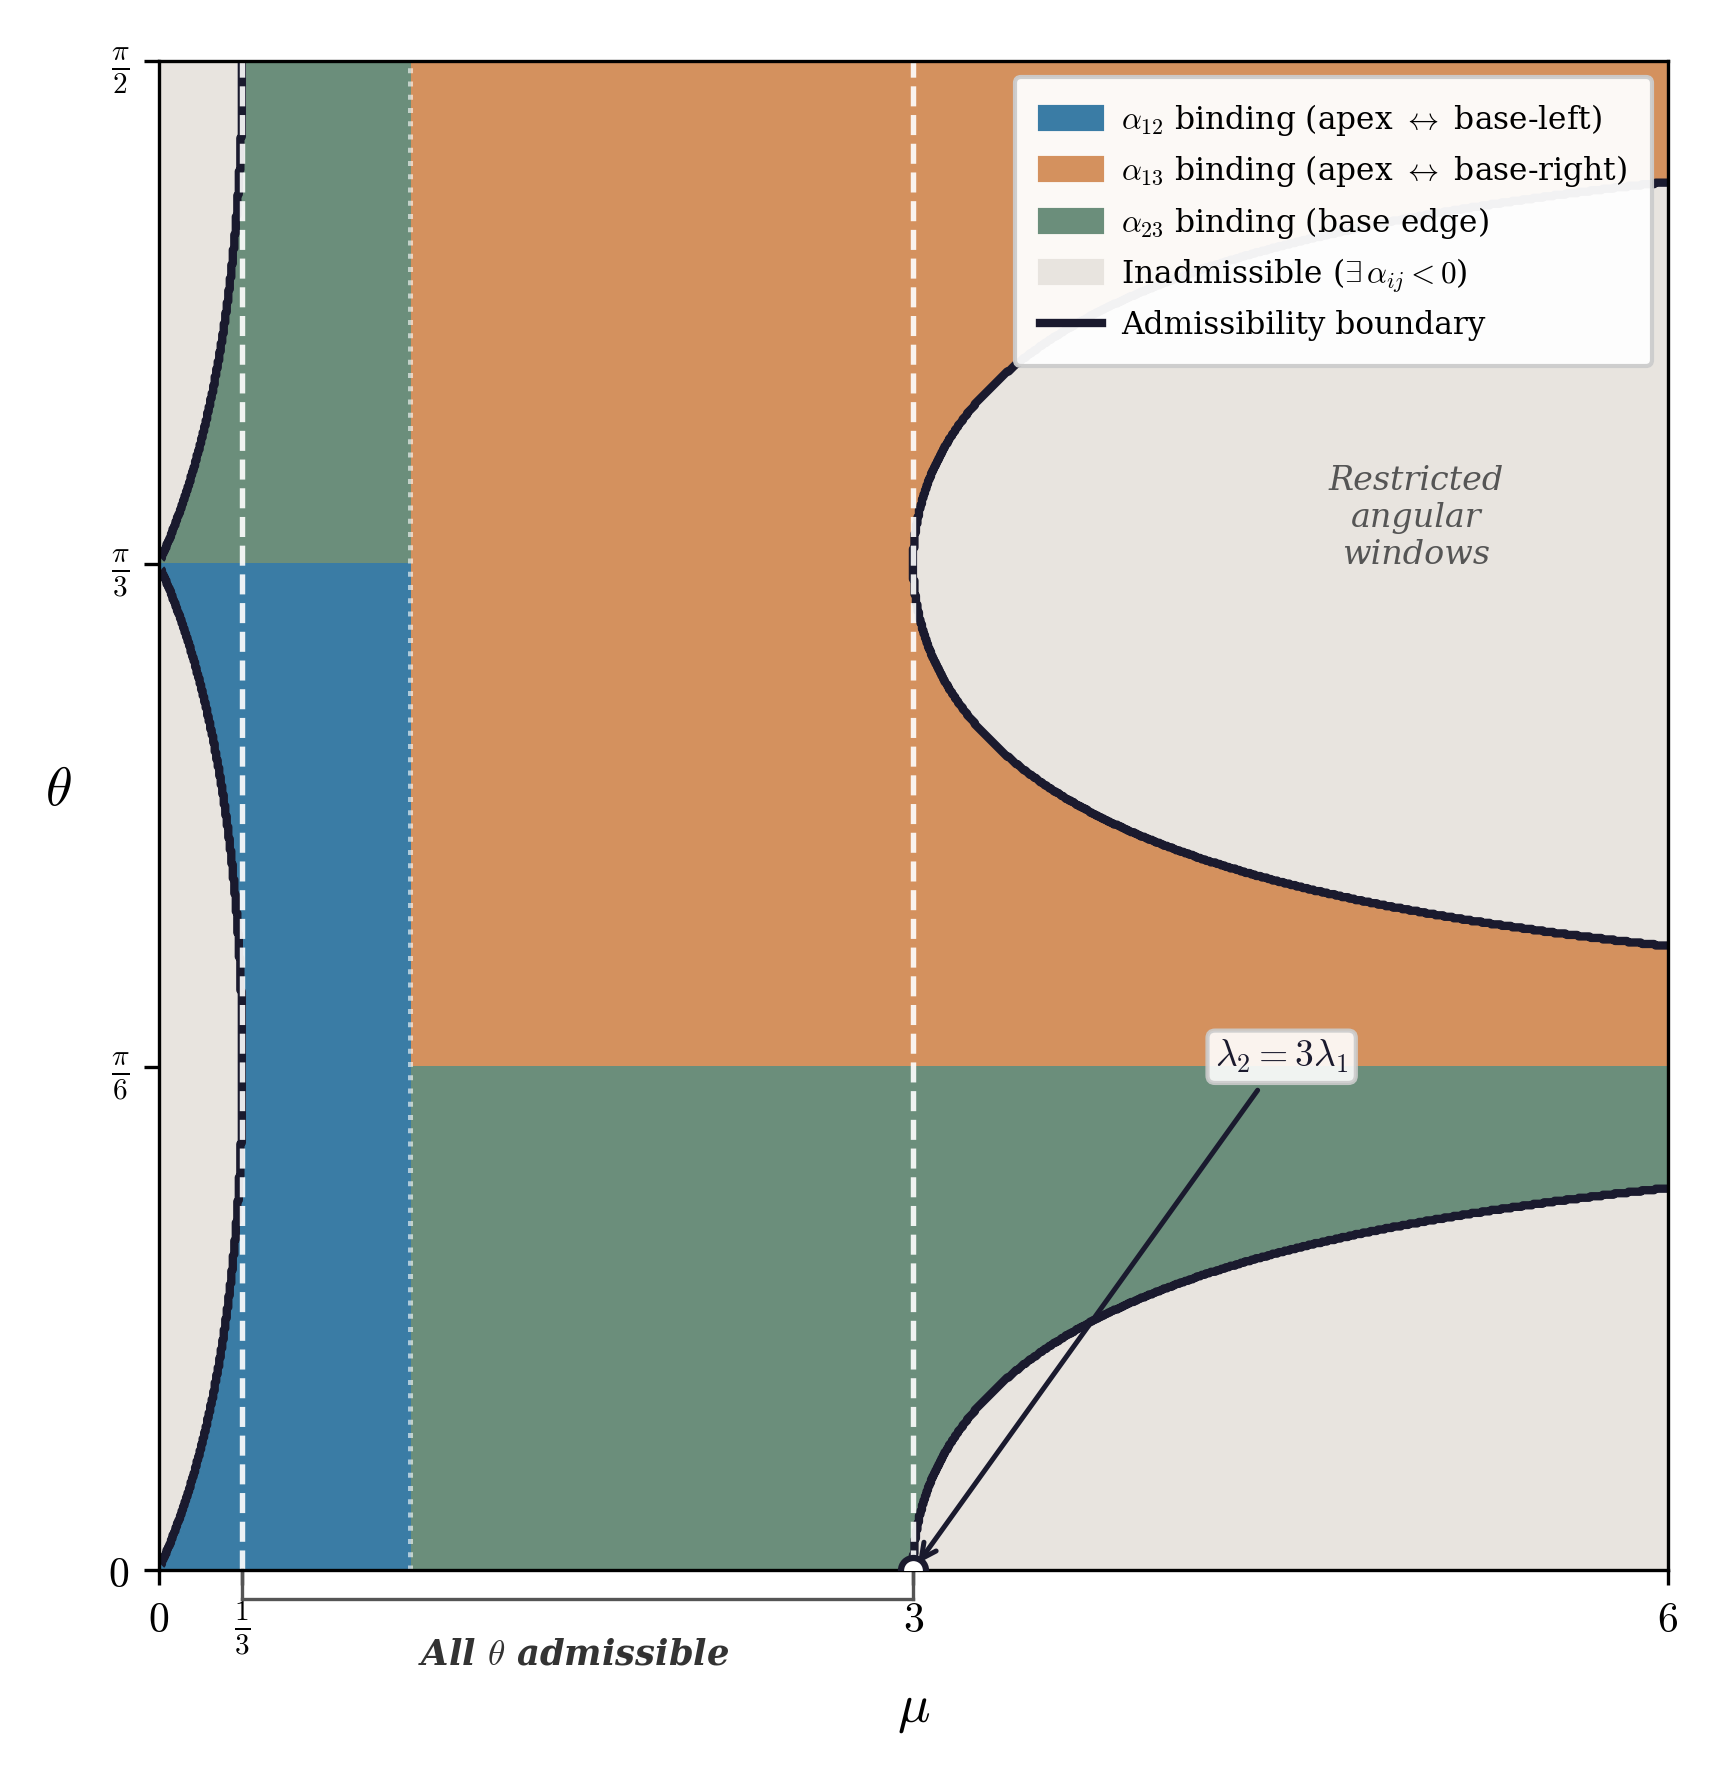
\includegraphics[width=0.5\linewidth]{../figures/figure_1_admissibility_binding}
\caption{Admissibility analysis for the equilateral triangle configuration
with rotational degree of freedom $\theta$ in the $\left(\mu,\theta\right)$
parameter space, where $\mu=\frac{\left|\lambda_{2}\right|}{\left|\lambda_{1}\right|}$
is the Hessian eigenvalue ratio.\textbf{}\protect \\
\textbf{(a)} Admissibility region (blue) defined by $\alpha_{12},\alpha_{13},\alpha_{23}\protect\geq0$.
Dashed red lines mark the critical values $\mu=\frac{1}{3}$ and $\mu=3$
between which all orientations $\theta\in\left[0,\pi/2\right]$ are
admissible. The point $\left(\mu,\theta\right)=\left(3,0\right)$
corresponds to the unrotated equilateral triangle requiring $\lambda_{2}=3\lambda_{1}$.\protect \\
\textbf{(b)} Identification of the tightest (binding) constraint at
each admissible point: red indicates $\alpha_{12}$ is smallest, orange
indicates $\alpha_{13}$, gray indicates $\alpha_{23}$. The boundary
between colored regions corresponds to the loci where two constraints
are simultaneously active.\protect \\
\textbf{(c)} Admissible $\theta$-ranges as a function of $\mu$,
constructed by sweeping the three nonnegativity constraints over $\mu\in\left(0,6\right)$.
Blue shading indicates admissible $\left(\mu,\theta\right)$ pairs;
this panel provides a complementary view of the same feasibility region
shown in (a).}
\label{fig:admissibility}
\end{figure}


\section{The Perturbation System}

\label{sec:perturbation}

We now extend the limiting configurations ($R=0$) to exact solutions
at finite energy ($R>0$). We focus on the equilateral triangle at
$\theta=0$.

\subsection{Formulation}

\label{subsec:formulation}

Write $\tilde{y}_{i}=\tilde{m}_{R}\,y_{i}+\delta y_{i}$ with $\delta y_{i}/\tilde{m}_{R}\to0$
as $R\to0$, where $\delta y_{i}\in\operatorname{span}\{\boldsymbol{r}_{1},\boldsymbol{r}_{2}\}$.
\begin{defn}[Perturbation system]
\label{def:Fi} Define 
\begin{equation}
F_{i}(\delta y,R)=\HV y_{i}+\HV\frac{\delta y_{i}}{\tilde{m}_{R}}-\sum_{k\in N_{i}}\frac{2Q_{R}\bigl(|\tilde{m}_{R}(y_{k}-y_{i})+\delta y_{k}-\delta y_{i}|\bigr)}{\norm{u_{R}}_{L^{2}}^{2}\,R^{4}\,|\tilde{m}_{R}(y_{k}-y_{i})+\delta y_{k}-\delta y_{i}|}\Bigl(y_{k}-y_{i}+\frac{\delta y_{k}-\delta y_{i}}{\tilde{m}_{R}}\Bigr).\label{eq:Fi-def}
\end{equation}
Extending by continuity to $R=0$: 
\begin{equation}
F_{i}(\delta y,0)=\HV y_{i}-\chi\sum_{k\in N_{i}}e^{-\ip{y_{k}-y_{i}}{\delta y_{k}-\delta y_{i}}}(y_{k}-y_{i}),\label{eq:Fi-zero}
\end{equation}
where $\chi$ is the overall interaction strength (Definition~\ref{def:chi}),
and the perturbed interaction coefficients are $\tilde{\alpha}_{ki}=e^{-\ip{y_{k}-y_{i}}{\delta y_{k}-\delta y_{i}}}$,
satisfying $\tilde{\alpha}_{ki}\chi\to\alpha_{ki}\chi$ as $\delta y\to0$.
Note that the constraint $\max_{k}\alpha_{ki}=1$ from~(\ref{eq:alpha-def})
normalizes $\chi$ to equal the total force from a nearest-neighbor
pair at minimum distance.

The Fr�chet derivative is 
\begin{equation}
D_{\delta y}F_{i}(\delta y,0)[w]=\chi\sum_{k\in N_{i}}\ip{w_{k}-w_{i}}{y_{k}-y_{i}}\,e^{-\ip{y_{k}-y_{i}}{\delta y_{k}-\delta y_{i}}}(y_{k}-y_{i}).\label{eq:Fi-deriv}
\end{equation}
\end{defn}

\subsection{Explicit solution at $R=0$}

\label{subsec:explicit}
\begin{prop}[Explicit solution]
\label{prop:explicit-soln} Define $\beta=\frac{1}{2}\ln\left(\frac{\alpha_{12}}{\alpha_{23}}\right)$
and $\gamma=\frac{2\beta}{3\sqrt{3}}$, where $\alpha_{12}=-\frac{\lambda_{2}}{3}$
and $\alpha_{23}=\frac{\lambda_{2}}{6}-\frac{\lambda_{1}}{2}$ are
the unperturbed coefficients. Then 
\begin{equation}
\delta y_{1}^{0}=-\gamma\,\boldsymbol{r}_{2},\qquad\delta y_{2,3}^{0}=\mp\beta\,\boldsymbol{r}_{1}+\frac{\gamma}{2}\,\boldsymbol{r}_{2}\label{eq:delta-y0}
\end{equation}
solves $F_{i}(\delta y,0)=0$ for $i=1,2,3$. 
\end{prop}
\begin{proof}
The perturbed interaction coefficients at $\delta y^{0}$ are (computed
by direct substitution): 
\begin{align*}
\tilde{\alpha}_{12}=\tilde{\alpha}_{13} & =e^{-\ip{y_{2}-y_{1}}{\delta y_{2}^{0}-\delta y_{1}^{0}}}=1,\\
\tilde{\alpha}_{23}=\tilde{\alpha}_{32} & =e^{-\ip{y_{3}-y_{2}}{\delta y_{3}^{0}-\delta y_{2}^{0}}}=\frac{\alpha_{23}}{\alpha_{12}}.
\end{align*}
The first follows from the fact that $\ip{y_{2}-y_{1}}{\delta y_{2}^{0}-\delta y_{1}^{0}}=0$
(which one verifies by substituting the explicit coordinates). The
second uses $\ip{y_{3}-y_{2}}{\delta y_{3}^{0}-\delta y_{2}^{0}}=2\beta=\ln\left(\frac{\alpha_{12}}{\alpha_{23}}\right)$.

Setting $\chi=-\frac{\lambda_{2}}{3}$ (the overall interaction strength
from Remark~\ref{rmk:alpha-convention}, equal to the combined force
coefficient $\hat{\alpha}_{12}$ of the apex--base edges), the system
$F_{i}(\delta y^{0},0)=0$ becomes 
\[
\HV y_{i}=\alpha_{12}\bigl[\tilde{\alpha}_{i1}(y_{1}-y_{i})+\tilde{\alpha}_{i,\text{other}}(y_{\text{other}}-y_{i})\bigr]
\]
for each $i$, which reduces to the original algebraic system~(\ref{eq:algebraic}).
Substituting the known values and simplifying component-wise confirms
$F_{i}=0$ for each $i$.

We also verify the center-of-mass condition: $\delta y_{1}^{0}+\delta y_{2}^{0}+\delta y_{3}^{0}=(0,0)$,
which is immediate from the definitions. 
\end{proof}

\subsection{Kernel of the linearization}

\label{subsec:kernel}
\begin{prop}[Nontrivial kernel]
\label{prop:kernel} The linearization $D_{\delta y}F_{i}(\delta y^{0},0)$
has a four-dimensional kernel 
\[
\Omega=\{(w_{1},w_{2},w_{3})\in(\R^{2})^{3}:\ip{w_{k}-w_{i}}{y_{k}-y_{i}}=0\;\;\forall\,i\neq k\}.
\]
This kernel contains the two-dimensional translational subspace $\{(v,v,v):v\in\R^{2}\}$
and two additional directions, including the rotational mode $w_{\mathrm{rot}}=\frac{d}{d\theta}y_{i}(\theta)\big|_{\theta=0}$. 
\end{prop}
\begin{proof}
The kernel condition $\ip{w_{k}-w_{i}}{y_{k}-y_{i}}=0$ for all neighbor
pairs gives three scalar constraints on $w\in\R^{6}$. Since $y_{3}-y_{2}=(y_{3}-y_{1})-(y_{2}-y_{1})$,
only two constraints are independent, so $\dim\Omega\geq6-2=4$.

To see that $\Omega\supseteq\{(v,v,v):v\in\R^{2}\}$: if $w_{1}=w_{2}=w_{3}=v$,
then $w_{k}-w_{i}=0$, so all inner products vanish. This is a 2D
subspace.

The quadratic form argument shows the inclusion is an equality: define
\[
\Phi=\sum_{i}w_{i}\cdot D_{\delta y}F_{i}(\delta y^{0},0)[w]=-\chi\sum_{\{i,k\}\in\text{edges}}\alpha_{ik}\bigl(\ip{w_{k}-w_{i}}{y_{k}-y_{i}}\bigr)^{2}.
\]
Since $\Phi\leq0$ and $\Phi=0$ implies each summand vanishes (as
$\alpha_{ik}>0$ for all edges of the equilateral triangle), the kernel
is precisely $\Omega$. Computing explicitly, $\dim\Omega=4$.

The rotational mode $w_{\mathrm{rot}}=(\frac{d}{d\theta}y_{i}(\theta)|_{\theta=0})_{i=1,2,3}=(-h,0;\;\frac{h}{2},-a;\;\frac{h}{2},a)$
lies in $\Omega$ since $\ip{w_{\mathrm{rot},k}-w_{\mathrm{rot},i}}{y_{k}-y_{i}}=0$
for all pairs (verified by direct computation). 
\end{proof}
\noindent\begin{rmk}\label{rmk:kernel-dim-new} The four kernel
dimensions decompose as follows. The two translational modes $\{(v,v,v):v\in\R^{2}\}$
span a $2$-dimensional subspace. The rotational mode $w_{\mathrm{rot}}$
accounts for one additional dimension. The remaining fourth direction
is a \emph{breathing mode}: it corresponds to a simultaneous dilation/contraction
of the triangle that preserves the kernel condition $\ip{w_{k}-w_{i}}{y_{k}-y_{i}}=0$.
Explicitly, one can verify that $w_{\mathrm{br}}=(y_{1}^{\perp},y_{2}^{\perp},y_{3}^{\perp})$,
where $y_{i}^{\perp}$ is the $90^{\circ}$ rotation of $y_{i}$ within
the $(\boldsymbol{r}_{1},\boldsymbol{r}_{2})$-plane, lies in $\Omega$
and is linearly independent of the translational and rotational modes.

The gauge-fixing conditions (G1)--(G2) remove the $\boldsymbol{r}_{1}$-translation
and the rotational mode, leaving a $2$-dimensional residual kernel
(the $\boldsymbol{r}_{2}$-translation and the breathing mode) that
must be handled by the parallel projection $P_{w}F$. \end{rmk}

\section{Kernel Resolution and Gauge-Fixing}

\label{sec:gauge}

The four-dimensional kernel $\Omega$ prevents a direct application
of the implicit function theorem (IFT) to continue solutions from
$R=0$ to $R>0$. Following the iterative kernel decomposition methodology
of~\cite{KirrNatarajan2018}, we decompose the reduced system into
projections perpendicular and parallel to $\Omega$.

\subsection{Projection decomposition}

\label{subsec:projections}

For $w\in\Omega$, define 
\[
P_{w}F(\delta y,R)=\sum_{i}\ip{w_{i}}{F_{i}(\delta y,R)}.
\]
We decompose $F$ into its perpendicular projection $P_{\perp}F$
(a vector-valued system on $\Omega^{\perp}$) and parallel projections
$P_{w}F$ for $w$ ranging over a basis of $\Omega$.

At $(\delta y^{0},0)$, the linearizations are: 
\begin{align}
D_{\delta y}P_{\perp}F\left(\delta y^{0},0\right)\left[\delta w\right] & =P_{\perp}\sum_{k\in N_{i}}\left\langle \delta w_{k}-\delta w_{i},y_{k}-y_{i}\right\rangle \,\tilde{\alpha}_{ik}\left(0\right)\,\chi\,\left(y_{k}-y_{i}\right),\label{eq:DPperp}\\
D_{\delta y}P_{w}F\left(\delta y^{0},0\right)\left[\delta w\right] & =\sum_{i}\left[\left\langle w_{i},\HV\delta w_{i}\right\rangle +\sum_{k\in N_{i}}\tilde{\alpha}_{ki}\left(0\right)\bigl(\left\langle w_{i},\delta y_{k}^{0}-\delta y_{i}^{0}\right\rangle \left\langle y_{k}-y_{i},\delta w_{k}-\delta w_{i}\right\rangle -\left\langle w_{i},\delta w_{k}-\delta w_{i}\right\rangle \bigr)\right].\label{eq:DPpar}
\end{align}


\subsection{Gauge-fixing constraints}

\label{subsec:gauge-fix}

To break the translational and rotational symmetries, we impose: 
\begin{enumerate}
\item[(G1)] $\delta y_{1}\perp\boldsymbol{r}_{1}$ (the first peak has no displacement
along $\boldsymbol{r}_{1}$), 
\item[(G2)] $(\delta y_{3}-\delta y_{2})\parallel\boldsymbol{r}_{1}$ (the base
of the triangle displaces only along $\boldsymbol{r}_{1}$). 
\end{enumerate}
These two scalar constraints remove 2 of the 4 kernel directions (one
translation component and the rotation mode), leaving a 2-dimensional
residual kernel corresponding to the remaining translation and the
breathing mode.

\subsection{Rotational equivariance at $R=0$}

\label{subsec:equivariance}
\begin{prop}[Family structure at $R=0$]
\label{prop:family} The one-parameter family of equilateral triangle
configurations $y_{i}(\theta)=R(\theta)y_{i}'$, $\theta\in[\theta_{\min},\theta_{\max}]$
(the admissible $\theta$-range from Proposition~\ref{prop:admissibility}),
generates a corresponding family of solutions $\delta y^{0}(\theta)$
of the system $F_{i}(\delta y,0)=0$. 
\end{prop}
\begin{proof}
For each admissible $\theta$, the base configuration $y_{i}(\theta)$
satisfies the algebraic system~(\ref{eq:algebraic}) with $\theta$-dependent
coefficients $\alpha_{12}(\theta),\alpha_{13}(\theta),\alpha_{23}(\theta)$
from~(\ref{eq:alpha12})--(\ref{eq:alpha23}). The explicit solution
construction of Proposition~\ref{prop:explicit-soln} applies at
each $\theta$, with $\beta\left(\theta\right)=\frac{1}{2}\ln\left(\frac{\alpha_{12}\left(\theta\right)}{\alpha_{23}\left(\theta\right)}\right)$
and $\gamma\left(\theta\right)=\frac{2\beta\left(\theta\right)}{3\sqrt{3}}$.
The resulting $\delta y^{0}\left(\theta\right)$ is smooth in $\theta$
since the $\alpha_{ki}\left(\theta\right)$ are smooth and positive
in the admissible range. 
\end{proof}
\begin{cor}
\label{cor:tangent-kernel} The tangent vector $\frac{d}{d\theta}\delta y^{0}\left(\theta\right)$
at each $\theta$ lies in the kernel $\Omega(\theta)$ of $D_{\delta y}F_{i}(\delta y^{0}(\theta),0)$.
This is the rotational mode $w_{\mathrm{rot}}(\theta)$. 
\end{cor}
\begin{proof}
Since $F_{i}(\delta y^{0}(\theta),0)=0$ holds for all admissible
$\theta$, differentiating with respect to $\theta$ gives 
\[
D_{\delta y}F_{i}(\delta y^{0}(\theta),0)\Bigl[\frac{d}{d\theta}\delta y^{0}(\theta)\Bigr]+\frac{\partial}{\partial\theta}\Bigl[F_{i}\bigl(\delta y^{0}(\theta),0\bigr)\Bigr]\bigg|_{\delta y\,\text{fixed}}=0.
\]
The second term accounts for the $\theta$-dependence of the base
configuration $y_{i}(\theta)$ and the coefficients $\alpha_{ki}(\theta)$;
it vanishes because the entire expression $F_{i}(\delta y^{0}(\theta),0)$
is identically zero in~$\theta$. Consequently, 
\[
D_{\delta y}F_{i}(\delta y^{0}(\theta),0)\Bigl[\frac{d}{d\theta}\delta y^{0}(\theta)\Bigr]=0,
\]
so $w_{\mathrm{rot}}(\theta)=\frac{d}{d\theta}\delta y^{0}(\theta)\in\Omega(\theta)$. 
\end{proof}

\subsection{Extension to $R>0$: invertibility of the gauge-fixed system}

\label{subsec:IFT}

\begin{conj}[Gauge-fixed invertibility]\label{conj:invertibility}
Under gauge-fixing conditions (G1)--(G2), the projected system 
\[
P_{\perp}F(\delta y,R)=0,\qquad P_{w}F(\delta y,R)=0\quad(w\in\Omega\setminus\operatorname{span}\{w_{\mathrm{trans}},w_{\mathrm{rot}}\})
\]
restricted to the gauge-fixed subspace $\{\delta y:\delta y_{1}\perp\boldsymbol{r}_{1},\;(\delta y_{3}-\delta y_{2})\parallel\boldsymbol{r}_{1}\}$
has an invertible linearization at $(\delta y^{0},0)$, and hence
the IFT yields a unique smooth branch $\delta y(R)$ for $R\in[0,\varepsilon)$.
\end{conj}

The conjecture is supported by the following partial result:
\begin{prop}[Center-of-mass identity]
\label{prop:sum-Fi} For any $\delta y=(\delta y_{1},\delta y_{2},\delta y_{3})$
and any $R\geq0$, 
\begin{equation}
\sum_{i=1}^{3}F_{i}(\delta y,R)=\HV\frac{\sum_{i}\delta y_{i}}{\tilde{m}_{R}}\,.\label{eq:sum-Fi-identity}
\end{equation}
In particular, $\sum_{i}F_{i}=0$ if and only if $\sum_{i}\delta y_{i}=0$
(the center-of-mass condition). The explicit solution $\delta y^{0}$
of Proposition~\ref{prop:explicit-soln} satisfies this condition,
and the gauge-fixing constraints \textup{(G1)--(G2)} are compatible
with~$\delta y^{0}$. 
\end{prop}
\begin{proof}
The interaction terms in $F_{i}$ (Definition~\ref{def:Fi}) involve
differences $(y_{k}-y_{i})$ and $(\delta y_{k}-\delta y_{i})/\tilde{m}_{R}$.
Each nearest-neighbor edge $\{i,k\}$ contributes to $\sum_{i}F_{i}$
through both the $F_{i}$ summand (with factor $y_{k}-y_{i}+(\delta y_{k}-\delta y_{i})/\tilde{m}_{R}$)
and the $F_{k}$ summand (with factor $y_{i}-y_{k}+(\delta y_{i}-\delta y_{k})/\tilde{m}_{R}$).
Since the scalar coefficient $\frac{2Q_{R}(|\tilde{y}_{k}-\tilde{y}_{i}|)}{\norm{u_{R}}_{L^{2}}^{2}R^{4}|\tilde{y}_{k}-\tilde{y}_{i}|}$
depends only on $|\tilde{y}_{k}-\tilde{y}_{i}|=|\tilde{y}_{i}-\tilde{y}_{k}|$,
these contributions are equal in magnitude and opposite in sign; hence
they cancel.

What remains from the Hessian terms is 
\[
\sum_{i=1}^{3}F_{i}(\delta y,R)=\sum_{i=1}^{3}\Bigl[\HV y_{i}+\HV\frac{\delta y_{i}}{\tilde{m}_{R}}\Bigr]=\HV\frac{\sum_{i}\bigl(\tilde{m}_{R}\,y_{i}+\delta y_{i}\bigr)}{\tilde{m}_{R}}\,.
\]
For the equilateral triangle, $\sum_{i}y_{i}=0$ by symmetry (the
centroid is at the origin), so $\sum_{i}F_{i}=\HV\,\bigl(\sum_{i}\delta y_{i}\bigr)/\tilde{m}_{R}$.
Since $\HV$ is invertible (Hypothesis~V3), $\sum_{i}F_{i}=0$ if
and only if $\sum_{i}\delta y_{i}=0$.

\smallskip{}
For the explicit solution: $\sum_{i}\delta y_{i}^{0}=(-\gamma\boldsymbol{r}_{2})+(-\beta\boldsymbol{r}_{1}+\frac{\gamma}{2}\boldsymbol{r}_{2})+(\beta\boldsymbol{r}_{1}+\frac{\gamma}{2}\boldsymbol{r}_{2})=\boldsymbol{0}$.

\smallskip{}
For the gauge-fixing compatibility: $\delta y_{1}^{0}=-\gamma\boldsymbol{r}_{2}$
has zero $\boldsymbol{r}_{1}$-component, so $\delta y_{1}^{0}\perp\boldsymbol{r}_{1}$
(condition G1). And $\delta y_{3}^{0}-\delta y_{2}^{0}=2\beta\boldsymbol{r}_{1}\parallel\boldsymbol{r}_{1}$
(condition G2). 
\end{proof}
\begin{rmk} The full resolution of Conjecture~\ref{conj:invertibility}
requires an explicit computation of the $4\times4$ matrix $D_{\delta y}(P_{\perp}F\oplus P_{\parallel}F)$
restricted to the gauge-fixed 4-dimensional subspace, and showing
its $2\times2$ restriction to $\Omega^{\perp}$ within the gauge-fixed
space is nonsingular. For the isotropic case $\mu=1$ ($\lambda_{1}=\lambda_{2}$),
the full continuous rotational symmetry $\HV=\lambda\,I$ implies
equivariance $F_{i}(R_{\omega}\delta y,R)=R_{\omega}F_{i}(\delta y,R)$
for all $\omega$, and the IFT applies on the quotient by the rotation
group. For anisotropic $\mu\neq1$, the equivariance is broken but
the family structure (Proposition~\ref{prop:family}) provides the
necessary tangent-space information. \end{rmk}

\section{Conclusion, Open Problems, and Acknowledgements}

\label{sec:conclusion}

We have carried out a complete finite-dimensional study of multi-peak
ground states for the nonlinear Schr�dinger equation 
\[
(-\Delta+V+E)\psi+\sigma|\psi|^{2p}\psi=0,\qquad E\to\infty,
\]
under Hypotheses~\ref{hyp:V1}--\ref{hyp:V4}. Our main results
are:
\begin{enumerate}
\item \textbf{Classification} (Theorem~\ref{thm:classification}). All
admissible multi-peak configurations near a non-degenerate local maximum
of $V$ are classified: collinear, isosceles triangle ($\lambda_{2}=3\lambda_{1}$),
equilateral triangle ($|\lambda_{2}/\lambda_{1}|\geq3$), and equilateral
with rotational freedom (Table~\ref{tab:summary}).
\item \textbf{Perturbation system} (Propositions~\ref{prop:explicit-soln}--\ref{prop:kernel}).
The system $F_{i}(\delta y,R)=0$ admits an explicit solution $\delta y^{0}$
at $R=0$, and the linearization has a four-dimensional kernel $\Omega$
(translations $+$ rotation $+$ breathing mode).
\item \textbf{Kernel resolution strategy} (Section~\ref{sec:gauge}). Gauge-fixing
conditions remove the translational and rotational freedom. The family
structure (Proposition~\ref{prop:family}) provides the tangent information,
and Conjecture~\ref{conj:invertibility} identifies the remaining
technical step. 
\end{enumerate}

\paragraph{Open problems.}

The following concrete, finite-dimensional problems remain:
\begin{enumerate}
\item \textbf{Prove Conjecture~\ref{conj:invertibility}} by computing
the linearized operator on the gauge-fixed subspace explicitly (a
$4\times4$ matrix computation) and verifying nonsingularity for $\mu>3$.
\item \textbf{Extend to all admissible $\theta$}. The current perturbation
analysis is carried out at $\theta=0$. Proposition~\ref{prop:family}
shows the family exists at $R=0$; extending to $R>0$ for all admissible
$\theta$ simultaneously requires uniform estimates.
\item \textbf{Stability.} Multi-peak branches with $M\geq2$ have at least
two negative directions in the linearized PDE operator~\cite{GrillakisShatahStrauss1987},
implying orbital instability. Adapting the asymptotic stability techniques
of~\cite{KirrZarnescu2007,KirrMizrak2008,KirrZarnescu2009,Kirr2016}
to multi-peak states remains open. 
\end{enumerate}
Once Conjecture~\ref{conj:invertibility} is resolved, the Lyapunov--Schmidt
machinery of~\cite{KirrNatarajan2018} lifts the finite-dimensional
solutions to exact multi-peak ground states of~(\ref{eq:NLS}) for
all sufficiently large energies $E$.

\paragraph{Acknowledgments}

The second author thanks Eduard Kirr for proposing this problem, for
many insightful discussions throughout the course of this research,
and for his academic guidance. This work was partially supported by
{[}DMS-XXXXXXX Placeholder etc.{]}.

\bibliographystyle{plain}
\bibliography{Research}


\appendix

\section{Notation Reference}

\label{app:notation}
\begin{center}
\begin{table}[H]
\centering
\begin{tabularx}{\columnwidth}{>{\raggedright\arraybackslash}Xl}
\toprule 
Symbol & Description\tabularnewline
\midrule 
$\psi_{E}:\mathbb{R}^{n}\to\mathbb{C}$ & Solution of~(\ref{eq:NLS}) at energy $E$\tabularnewline
$V:\mathbb{R}^{n}\to\mathbb{R}$, $\HV\left(x_{0}\right):\mathbb{R}^{n}\to\mathbb{R}^{n\times n}$ & External potential and its Hessian at $x_{0}$\tabularnewline
$\sigma\in\mathbb{R}^{+}$, $p$ & Nonlinearity coefficient and nonlinearity exponent\tabularnewline
$\lambda_{i}$, $\boldsymbol{r}_{i}$ & Eigenvalues/eigenvectors of $\HV(x_{0})$; $\lambda_{i}<0$\tabularnewline
$\mu=\frac{\left|\lambda_{2}\right|}{\left|\lambda_{1}\right|}$ & Eigenvalue ratio\tabularnewline
$E\in\mathbb{R}^{+}\cup\left\{ 0\right\} $, $R=E^{-\frac{1}{2}}$ & Energy parameter and rescaling parameter; $R\to0$ as $E\to\infty$\tabularnewline
$u_{E}\left(x\right)=E^{-\frac{1}{2p}}\psi_{E}\left(E^{-\frac{1}{2}}x\right)$ & Rescaled solution\tabularnewline
$Q_{R}(z)$ & Interaction functional (Definition~\ref{def:interaction})\tabularnewline
$\alpha_{ki}$ & Interaction coefficient (Definition~\ref{def:interaction}); $0\leq\alpha_{ki}\leq1$\tabularnewline
$\chi$ & Overall interaction strength (Definition~\ref{def:chi})\tabularnewline
$m_{R}$ & Minimum inter-peak distance: $m_{R}=\min_{i\neq j}\left|z_{i}\left(R\right)-z_{j}\left(R\right)\right|$\tabularnewline
$s_{i}=Rz_{i}-x_{0}$ & Displacement of $i-$th peak from critical point $x_{0}$\tabularnewline
$y_{i}=\lim_{R\to0}\frac{s_{i}}{Rm_{R}}$ & Limiting peak positions\tabularnewline
$\delta y_{i}\in\text{span}\left\{ \boldsymbol{r}_{1},\boldsymbol{r}_{2}\right\} $ & Perturbation of peak $i$\tabularnewline
$F_{i}(\delta y,R)$ & Perturbation system (Definition~\ref{def:Fi})\tabularnewline
$\tilde{\alpha}_{ki}=e^{-\left\langle y_{k}-y_{i},\delta y_{k}-\delta y_{i}\right\rangle }$ & Perturbed interaction coefficient ($R=0$)\tabularnewline
$\tilde{y}_{i}=\tilde{m}_{R}y_{i}+\delta y_{i}$ & Perturbed peak position; $\frac{\delta y_{i}}{\tilde{m}_{R}}\to0$
as $R\to0$\tabularnewline
$\Omega$ & Kernel of $D_{\delta y}F_{i}(\delta y^{0},0)$ (Proposition~\ref{prop:kernel})\tabularnewline
$\theta$ & Rotation angle of equilateral triangle\tabularnewline
$\nu(\mu),\varphi(\mu)$ & Admissibility functions (Definition~\ref{def:nu-phi})\tabularnewline
$u_{R}$ & Profile solving $(-\Delta+R^{2}V(x_{0})+1)u+\sigma|u|^{2p}u=0$; unique
positive radial solution\tabularnewline
$h_{R}$ & Remainder: $u_{E}=\sum_{i}u_{R}(\cdot-z_{i})+h_{R}$, with $\|h_{R}\|_{H^{1}}\to0$\tabularnewline
$N_{i}$ & Nearest-neighbor set: $N_{i}=\{k:|y_{k}-y_{i}|=1\}$\tabularnewline
$\hat{\alpha}_{ki}=\alpha_{ki}\chi$ & Combined force coefficient (Remark~\ref{rmk:alpha-convention})\tabularnewline
$\beta,\gamma$ & Perturbation parameters (Proposition~\ref{prop:explicit-soln})\tabularnewline
$P_{\perp},P_{w}$ & Projections onto \$\tabularnewline
$w_{\mathrm{rot}},w_{\mathrm{br}}$ & Rotational and breathing kernel modes (Remark~\ref{rmk:kernel-dim-new})\tabularnewline
\bottomrule
\end{tabularx}

\caption{Table of commonly used symbols}
\end{table}
\par\end{center}

\begin{center}
%
\par\end{center}
\end{document}
